\documentclass[doc]{apa6}

\usepackage[english]{babel}
\usepackage[utf8x]{inputenc}
\usepackage{amsmath}
\usepackage{graphicx}
\usepackage{apacite}
\usepackage{amsfonts}
\usepackage{url}
\usepackage{tikz}
\usepackage{listings}
\usepackage{enumitem}
\usepackage{subfigure}
\usetikzlibrary{bayesnet}
\usepackage{bm}
\usepackage{cprotect}
\lstset{
    language=C,
    basicstyle=\small
}


%\usepackage[style=apa,sortcites=true,sorting=nyt,backend=biber]{biblatex}
%\DeclareLanguageMapping{american}{american-apa}

  \title{Warm (for Winter): Inferring comparison classes for scalar adjectives}
    \author{Michael Henry Tessler\textsuperscript{1,2} and Noah D. Goodman\textsuperscript{2}}
    \date{}
  
\shorttitle{ Inferring comparison classes}
\affiliation{
\vspace{0.5cm}

\textsuperscript{1}Department of Brain and Cognitive Sciences, Massachusetts Institute of Technology \\\textsuperscript{2}Department of Psychology, Stanford University}
\keywords{comparison class; pragmatics; Rational Speech Act; Bayesian cognitive model; Bayesian data analysis\newline\indent Word count: X}
\makeatletter
\newcommand\LastLTentrywidth{1em}
\newlength\longtablewidth
\setlength{\longtablewidth}{1in}
\usepackage{tabularx}
\usepackage{multicol}
\usepackage{wrapfig}
\usepackage{gensymb}
\usepackage{tikz}
\usepackage{caption}
\usepackage{booktabs}


% these packages are needed to insert results 
% obtained from R into the LaTeX document
\usepackage{pgfplotstable}
\usepackage{csvsimple}
\usepackage{siunitx}

\definecolor{Red}{RGB}{255,0,0}
\definecolor{Green}{RGB}{10,200,100}
\definecolor{Blue}{RGB}{10,100,200}
\definecolor{Orange}{RGB}{255,153,0}

\newcommand{\denote}[1]{\mbox{ $[\![ #1 ]\!]$}}
\newcommand*\diff{\mathop{}\!\mathrm{d}}
\newcommand{\red}[1]{\textcolor{Red}{#1}}  
\newcommand{\ndg}[1]{\textcolor{Green}{[ndg: #1]}}  
\newcommand{\mht}[1]{\textcolor{Blue}{[mht: #1]}}  
\newcommand{\mlb}[1]{\textcolor{Orange}{[mlb: #1]}}

% set the name of the folder in which the CSV files with 
% information from R is stored
\newcommand{\datafoldername}{csv_data_4_tex}

% the following code defines the convenience functions
% as described in the main text below

% rlgetvalue returns whatever is the in cell of the CSV file
% be it string or number; it does not format anything
\newcommand{\rlgetvalue}[4]{\csvreader[filter strcmp={\mykey}{#3},
             late after line = {{,}\ }, late after last line = {{}}]
            {\datafoldername/#1}{#2=\mykey,#4=\myvalue}{\myvalue}}

% rlgetvariable is a shortcut for a specific CSV file (myvars.csv) in which
% individual variables that do not belong to a larger chunk can be stored
\newcommand{\rlgetvariable}[1]{\csvreader[]{\datafoldername/myvars.csv}{#1=\myvar}{\myvar}\xspace}

% rlnum format a decimal number
\newcommand{\rlnum}[2]{\num[output-decimal-marker={.},
                             exponent-product = \cdot,
                             round-mode=places,
                             round-precision=#2,
                             group-digits=false]{#1}}

\newcommand{\rlnumsci}[2]{\num[output-decimal-marker={.},
                          scientific-notation = true,
                             exponent-product = \cdot,
                             round-mode=places,
                             round-precision=#2,
                             group-digits=false]{#1}}

\newcommand{\rlgetnum}[5]{\csvreader[filter strcmp={\mykey}{#3},
             late after line = {{,}\ }, late after last line = {{}}]
            {\datafoldername/#1}{#2=\mykey,#4=\myvalue}{\rlnum{\myvalue}{#5}}}

\newcommand{\rlgetnumsci}[5]{\csvreader[filter strcmp={\mykey}{#3},
             late after line = {{,}\ }, late after last line = {{}}]
            {\datafoldername/#1}{#2=\mykey,#4=\myvalue}{\rlnumsci{\myvalue}{#5}}}

\newcommand{\lmresults}[2]{\(\beta = \rlgetnum{#1}{Rowname}{#2}{Estimate}{3}\), t\((\rlgetnum{#1}{Rowname}{#2}{df}{0}) = \rlgetnum{#1}{Rowname}{#2}{t.value}{2}, p = \rlgetnum{#1}{Rowname}{#2}{Pr...t..}{3}\)}

\newcommand{\brmresults}[2]{\(\beta = \rlgetnum{#1}{Rowname}{#2}{Estimate}{3}\) (\rlgetnum{#1}{Rowname}{#2}{l.95..CI}{3}, \rlgetnum{#1}{Rowname}{#2}{u.95..CI}{3})}

\newcommand{\hdiresults}[2]{\rlgetnum{#1}{param_name}{#2}{MAP}{2} (\rlgetnum{#1}{param_name}{#2}{cred_lower}{2}, \rlgetnum{#1}{param_name}{#2}{cred_upper}{2})}

\authornote{Correspondence concerning this article should be addressed to Michael
Henry Tessler, Department of Brain and Cognitive Sciences, Building 46, Room 3027, Massachusetts Institute of Technology, 77 Massachusetts Avenue, Cambridge, MA 02139.
E-mail: tessler@mit.edu}

\abstract{
The meaning of an utterance can change depending on the context. Yet,
what counts as context is often only implicit in everyday
conversation. The utterance ``it's warm outside'' signals that the temperature outside is relatively high, but the temperature could be high relative to a number of different \emph{comparison classes}: other days of the year, other weeks, other seasons, etc... 
Theories of context-sensitive language use agree that the comparison class is a crucial feature of meaning understanding, but little is known about how a listener decides upon a comparison class.
We extend a Bayesian model of pragmatic reasoning to be able to reason flexibly about the comparison class intended by the speaker and test the qualitative predictions of this model using a large-scale free-production experiment.
%\ndg{awk:}
We introduce a hybrid experimental-Bayesian data analytic approach to examine the quantitative predictions of model, finding that usage frequency and a preference for basic-level categories are two main contributors to comparison class inference.
%We present free-production and forced-choice experiments showing reliable patterns of comparison class inference.
%The patterns of inference we observe are consistent with a model of Bayesian reasoning about the likely comparison class, which we incorporate into a probabilistic model of adjective interpretation, furthering the breadth of computational models of language understanding. 
The methods and results we present open the door to studying richer aspects of context-sensitive language understanding.
%We test the qualitative predictions of the model in a free production experiment and use a forced-choice version of the task to test the finer-grained, quantitative predictions. 
%The resolution of a comparison class requires not only reasoning about what is likely to be the case but also what would be informative to talk about, thus incorporating comparison class inference into the larger study of pragmatic reasoning.
}



\begin{document}
\maketitle



\section{Introduction}

%A man with a height of 5'2'' is short. 
%A 6'1'' man is not short; that is, unless the man is a basketball player; they could be short for a basketball player.


A 75\degree F (24\degree C) day is warm. A 50\degree F (10\degree C) day is not. That is, unless it's Winter; 50\degree F could be warm for Winter. \emph{Warm} is a relative adjective, and its felicity depends upon what a speaker uses as a basis of comparison---the \emph{comparison class} (e.g., warm relative to days in Winter~vs.~days in other seasons). Comparison classes are necessary for understanding relative adjectives  like \emph{warm} or \emph{tall} \cite{cresswell1976semantics, klein1980semantics, kennedy2005scale, bale2008universal, Bale2011, Solt2009}; in fact, comparison classes can be deployed in any linguistic expression that conveys something relative (\emph{relative to what?}), including vague quantifiers \cite<e.g., ``He ate a lot of burgers'' [\emph{relative to a typical person}];>{Scholler2017} and generic sentences \cite<e.g., ``Dogs are friendly'' [\emph{relative to other animals}];>{Tessler2019psychrev}.
Interpreting the meaning of an utterance by appealing to a comparison class is a case study in the larger project of understanding how human listeners use context to make sense of the words they hear.
The problem with comparison classes, as with notions of context more generally, is that they are almost never described explicitly (e.g., most speakers would probably articulate \emph{he's tall for person} as ``He's tall'').

%The particular comparison class that a speaker uses in generating in an utterance, however, is almost never actually articulated.
%In most contexts, the utterance .
The fact that comparison classes often go unsaid gives rise to an inferential problem for listeners.
Any particular referent of discourse can be conceptualized or categorized in multiple ways, giving rise to multiple possible comparison classes. 
A day in January is also a day of the year; if a listener hears ``It's warm'', it could be \emph{warm in comparison to the last week}, \emph{warm for the season}, or \emph{warm relative to other seasons}; it could also be \emph{warm for Boston}, \emph{warm for the northeast USA}, \emph{warm for a place with currently six inches of snow on the ground}, among an infinity of possibilities.
Furthermore, the connection between inferring the comparison class and theories of adjective meaning remains obscure because models of reasoning developed in psychology rarely talk to models of semantic meaning developed in linguistics.
%Theoretical work in semantics has instead focused on how information from an already determined comparison class is integrated with a compositional semantics and which representations might be preferred \cite{Bale2011, Solt2009}.

On the empirical side, the question of how listeners decide upon the comparison class has also received little systematic attention.
Instead, empirical work with adults and children has primarily interrogated how judgments and interpretations for relative adjectives like \emph{dark} or \emph{tall} depend upon statistical details of a pre-determined comparison class  \cite{Barner2008, Qing2014, Schmidt2009, Solt2012}.
Indirect evidence that the comparison class can be flexibly adjusted comes from studies with young children, which find that a directly-modified noun phrase (\emph{big pimwit}) can be used to constrain what objects goes go into the comparison class: What counts as a \emph{tall pimwit} (a novel category) depends on the distribution of heights of \emph{pimwits} and not the heights of other categories like \emph{daxes} \cite{Barner2008}. 
Additionally, strong linguistic and perceptual cues can also provide a signal to children as young as 2-and-a-half that the comparison class can change \cite<e.g., an objectively small mitten can be \emph{big} relative to the tiny mittens on the table;>{Ebeling1988, Ebeling1994}.
But, direct evidence that the comparison class can be flexibly adjusted based on systematic principles and the parameters that guide and constrain these inferences has yet to be uncovered.

%Thus, comparison classes are central to human understanding of relative statements and from the point at which children acquire the meaning for a relative adjective like ``big'', they already understand that the meaning can change with the comparison class.

%The hypothesis space of possible comparison classes is unbounded and deciding what goes into the hypothesis space is probably tantamount to the development of a general theory of concepts.
%Once a hypothesis space is determined, however, a listener still must decide which amongst multiple possible comparison classes a speaker intends (e.g., \emph{warm for winter} or \emph{warm for the year}). 
%It is this aspect of the problem---lying between a theory of concepts (which generates possible comparison classes) and natural language (how relative statements are interpreted)---that we bring light to in this paper. 

In this paper, we demonstrate one systematic aspect of comparison class inference: dependence on background knowledge about categories and properties.
We show that the problem of comparison class inference is one of pragmatic inference, which we 
%by weighting the prior probability of a comparison class with the likelihood that a speaker would use the adjective heard to describe the referent given that comparison class.
demonstrate in a computational model of pragmatic reasoning \cite<a Rational Speech Act model;> {Frank2012, Goodman2016, scontras2017probabilistic}. 
The model derives an intuitive interaction between a listener's general expectations about the referent (e.g., winter days are cold; summer days are warm) and the polarity of the adjective heard (e.g., \emph{warm}, \emph{cold}).
When the adjective is inconsistent with the listener's general expectations (e.g., the day in winter is warm), listeners should prefer a relatively subordinate comparison class (e.g., \emph{warm for winter}), whereas when the adjective is consistent with general expectations (e.g., the day in winter is cold), listeners should prefer a relatively superordinate comparison classes (e.g., \emph{cold for the year}). 
We show formally that this inference relies upon a sophisticated pragmatic mechanism: A listener uses their knowledge of the specific category (e.g., winter) to guide their expectations of what is likely to be true in the world, while simultaneously imagining how a speaker would behave given a different comparison class (e.g., what a speaker would say given the comparison class of \emph{days of the year}). 
We test this hypothesis in a large-scale, pre-registered, free-production experiment in which participants are free to come up with a preferred comparison class of their choosing. 

%Intuitively, the comparison class is not a fixed property of the referent nor the referent--predicate pair. 
%A ``tall basketball player'' might be tall for a basketball player or just tall for a person. 
%We propose a simple hypothesis about how comparison classes are determined
%\mht{i wonder if we should have this paragraph here at all... it kind of breaks the flow. we could just do quantitative modeling, and put this in the discussion section. alternatively, we could double down on this paragraph and make it more clear that this is one of the contributions of this paper. ``In addition to a model of comparison class inference and novel systematic empirical data about comparison class, we introduce a novel data analytic approach...''}
%The model we propose is quantitative in nature and thus, can predict graded inferences about comparison class as a result of background knowledge.  
%Background knowledge for language understanding models is often measured empirically by having participants estimate relevant quantities and probabilities \cite<e.g., plausible temperatures of days in winter, summer, etc...;>{Franke2016}.
%These explicit prior elicitation techniques are limited, however, to domains where participants have an accurate representation of the underlying scale (e.g., temperature); many domains can be reasoned about intuitively (e.g., the loudness of a diesel engine~vs.~an electric car) without a clear representation of the underlying scale (e.g., how many decibels is the typical sound of a diesel engine?).
%For this reason, we take a different approach: We utilize the productivity of our computational model to predict data from a related language experiment (truth judgments about adjectives) and synthesize the two data sets using a Bayesian data analytic model, wherein the parameters that govern background knowledge in the pragmatics models are constrained by both data sets.
%This joint data modeling provides a way to pin-down model parameters governing background knowledge by asking participants only simple, natural language questions, while also holding the cognitive models to the high standard of predicting data from multiple experiments using the same parameters.


%with a Bayesian data analytic approach 
%\ndg{the following is hard to follow. i'd suggest moving diascussion of 'descriptive bayesian' to discussion and here say more intuitively what we do..}
%We embed our model of pragmatic reasoning in a Bayesian data-analytic model where the parameters that govern background knowledge in the pragmatics model are inferred from the experimental data, a kind of \emph{descriptive Bayesian} modeling \cite{tauber2017}.
%We go further, however, than merely asking what background knowledge would account for comparison class inferences; we harness the productivity of natural language and the Rational Speech Act modeling framework to predict data from a related language experiment (truth judgments about adjectives) that relies upon the same background knowledge. 

%Deciding on the relevant comparison class is a case study in the larger question of inferring the appropriate aspects of context for interpreting an utterance.  


%We suggest this method
%We find that the comparison class can be flexibly adjusted based on prior knowledge, which our model can predict with high quantitative accuracy. 
%\red{[zoom back out. bigger picture.?]}

% listeners will flexibly adjust the comparison class when an adjective signals a degree (e.g., temperature) that is \emph{a priori} consistent with the listener's knowledge of the referent (e.g., as a member of a category that generally has a high or low temperature), the comparison class is likely to be a relatively general category (e.g., a basic or superordinate level category), whereas when the adjective signals a degree inconsistent with the listener's prior beliefs about the referent, the comparison class is likely to be a more specific (e.g., subordinate level) category.\footnote{Here, \emph{generally consistent} means generally high or low relative to a basic-level or superordinate level category that has some non-negligible probability of being a comparison class.}


%We explore such a hypothesis in this paper.
%The prior distribution over comparison classes is a theoretical object of interest in its own right---in its most general form, it is a probability distribution over possible contexts---and we will only begin to understand this distribution's properties via our experiments and model.%  of a comparison class is a 

%For example, in Winter, hearing \emph{it's warm} should signal \emph{warm for winter} (subordinate comparison class), while hearing \emph{it's cold} signals \emph{cold for the year} (a more basic or superordinate class). 
%The opposite relationship should hold in summer, where \emph{it's cold} should signal cold \emph{for summer} more so than \emph{it's warm}. 
%We describe in detail the mechanism behind this inference, formalized in a probabilistic model of language understanding, which in turn generates quantitative predictions that depend on background knowledge about categories and their properties. 
%We test the qualitative predictions in a large-scale free-production task where participants are asked to infer the comparison class the speaker had in mind. 

%This work provides 
%\red{We find X... [zoom back out. big picture] }

%This inference results from pragmatic reasoning and is not predicted by the alternative, non-pragmatic Bayesian model.
%These predictions fall out of a Rational Speech Act (RSA) model for gradable
%adjectives \cite{Lassiter2013, Lassiter2017}, extended to flexibly
%reason about the implicit comparison class. 

% a result of the \emph{a
%priori} probability of different temperatures in different seasons: In
%winter, temperatures are relatively low, and thus it is unlikely to
%actually be \emph{warm for the year}. 
%In addition, regardless of the
%season and the adjective (e.g., ``warm'' or ``cold''),
%listeners prefer comparison classes that are relatively specific (e.g.,
%relative to \emph{the current season} as opposed to \emph{the whole
%year}); more specific comparison classes have lower variance, and a
%vague adjectives like \emph{warm} carries more information when it is
%interpreted with respect to a lower variance comparison class. 

%\textcolor{Blue}{[mht: move to end of first expt]}
%
%The model's quantitative predictions can be generated by explicitly
%specifying the interlocutors' relevant prior knowledge (e.g., beliefs
%about temperatures). The current methodological standard is to measure
%beliefs by having participants estimate quantities or give likelihood
%judgments \cite{Franke2016}. We pursue a different methodology. The
%RSA model captures a productive fragment of natural language; thus, it
%makes predictions about a related natural language task (Expt. 2).
%Critically, we can use the model to predict natural language judgments
%that require the \emph{same prior knowledge} as in Expt. 1 and use
%Bayesian data analysis to jointly infer the shared priors. This approach
%harnesses the productivity of language into experiment design and allows
%us to reconstruct priors without having participants engage in
%challenging numerical estimation tasks.

\section{Computational Model}

%To explicate our model, we use the running example of hearing a basketball player described as either \emph{tall} or \emph{short} (Figure \ref{fig:modelCartoon}). 
%The guiding intuition that our model tries to explain is that when the basketball player is described as \emph{short}, it is likely that the comparison class intended by the speaker is the subordinate-level category (i.e., \emph{short for a basketball player}). 
%On the other hand, when the basketball player is described as \emph{tall}, the comparison class intended by the speaker is likely to be the more general category (i.e., \emph{tall for a person}).
%The opposite pattern should follow for a member of a category that is generally short, such as a jockey: \emph{he's short} should mean \emph{short for a person}, while \emph{he's tall} should signal \emph{tall for a jockey}.
%Though an intuitive inference, 
Here we articulate the computations that underly comparison class inference and how that inference interfaces with standard semantic theories of adjective meaning.
%We develop a computational model that integrates general purposes reasoning capabilities with a semantic model of adjective meaning. 
When interpreting an adjective utterance $u$ without an explicit comparison class (e.g., \emph{he's tall}), a listener is faced with the joint inference problem of determining the degree being described by the adjective $x$ (e.g., the height of the referent) and the comparison class $c$ assumed by the speaker when producing their utterance.
We assume the listener $L_1$  uses their knowledge of the referent $k$ (e.g., the category membership of the referent such as the referent is the basketball player) to both guide their expectations about the degree $x$ (e.g., the plausible height of the referent) as well as the hypothesis space of comparison classes $c$. 
With a Bayesian formulation, a listener combines these prior expectations with the likelihood that a speaker would use an adjective to describe a member of a particular category.\footnote{We use the male pronoun to refer to the listener and the female pronoun to refer to the speaker.}

%To explicate our model, we use the running example of hearing a basketball player described as either \emph{tall} or \emph{short} (Figure \ref{fig:modelCartoon}). 


%This inference is a result of the adjective \emph{short} conflicting with the general expectation that basketball players are tall people.
%Thus, 


%More generally, when an adjective conflicts with a listener's \emph{general expectations} about members of a category (e.g., \emph{short} described of a basketball player; general expectation: basketball players are tall), listeners should accommodate this utterance by positing a more specific comparison class (e.g., \emph{short for a basketball player}). 
%Our model grounds the \emph{general expectations} a listener would have about members of the category are, in fact, an interpretation of the scalar adjective under a basic or superordinate-level class (e.g., basketball players tend to be tall people).


% predicted when the basketball player is described as \emph{short} (i.e., more likely to be a \emph{short basketball player} than a \emph{short person}).


%The basic intuition that the model formalizes is that, when describing the height of a basketball player, a speaker is more likely to say \emph{he's a tall person} than \emph{he's a tall basketball player} because it is a more likely state of affairs given distributional knowledge of the heights of people and the heights of basketball players. 
%A listener then uses this knowledge of the speaker to infer the unsaid comparison class when the speaker says only: \emph{he's tall}.
%
%Finally, the same adjectives used to describe a jockey should invoke the opposite inferences (i.e., \emph{tall} $\rightarrow$ \emph{tall jockey}; \emph{short} $\rightarrow$ \emph{short person}).

%\subsection{Model specification}


\begin{align}
L_1(x, c \mid u, k) &\propto S_1(u \mid x, c) \cdot P(x \mid k) \cdot P(c \mid k) \label{eq:L1a} 
\end{align}
%

Eq. \ref{eq:L1a} describes a pragmatic listener $L_1$ updating his beliefs about the degree $x$ and the comparison class $c$ by assuming that the speaker $S_1$ intentionally produced an adjectival utterance $u$ so that she could communicate about the degree (e.g., height).
%The lis in this case is assuming , assuming the comparison class, 
The hypothesis space of comparison classes $P(c \mid k)$ is assumed to be in common ground, constrained by prior knowledge and common knowledge about the situation (e.g.,~that the referent is a basketball player).
Though comparison classes can be constructed in various ways, including sets of objects in the perceptual environment (e.g.,~\emph{big relative to these other things}) or from hypothetical functions of an object \cite<e.g., \emph{the shirt is big for the doll;}>{Ebeling1994}, we restrict our analysis to a hypothesis space of comparison classes constructed out of a taxonomic hierarchy of the subordinate category to which the referent belongs (i.e., \emph{conceptual comparison classes}, e.g., a basketball player is a person; Figure \ref{fig:modelCartoon}A). The hypothesis space of degrees (e.g., heights) is given by the semantics of the adjectives (e.g., \emph{tall} $\rightarrow$ height) and is also informed by the category membership of the referent $k$ (e.g., that the referent is a basketball player).\footnote{
More generally, the hypothesis space of comparison classes is constrained by the shared beliefs of the speaker and listener: A listener will not assume the speaker is using a comparison class about which the speaker is ignorant, and a listener cannot construct a comparison class from information about which they are ignorant. By contrast, expectations about the degree value for the referent (e.g., the referent's height) will be guided by the totality of the listener's beliefs --- both those shared with the speaker and the listener's private beliefs. For example, if the listener had private knowledge that the person in question was taking a growth-stunting medication, they would use that knowledge to guide their predictions about that person's height, though if the listener knew that the speaker did not know about the growth-stunting medication, that information would not enter in the hypothesis space of comparison classes. Formally, this more general model would be given by: \begin{align}
L_1(x, c \mid u, f, g) &\propto S_1(u \mid x, c) \cdot P(x \mid f, g) \cdot P(c \mid f) \label{eq:L1} 
\end{align}
\noindent where $f$ denotes the beliefs shared between speaker and listener, and $g$ denotes the listener's private beliefs. Since our paradigm does not distinguish between these kinds of beliefs, we use a reduced-form of the model, where beliefs are represented by a single variable $k$ and can be thought of as the most specific relevant category information about the referent (e.g., the referent is a basketball player).
}

Following work in the Rational Speech Act modeling framework \cite{Frank2012, Goodman2016, scontras2017probabilistic}, the speaker $S_1$ in this model is a soft-max rational agent (with degree of rationality $\alpha$) who produces utterances in order to convey information about the degree $x$ to a listener $L_0$ who knows the comparison class, while also taking into account the cost of the utterance $u$.\footnote{For simplicity, for all of our qualitative and quantitative modeling, we assume no difference in production cost for different utterances. Hence, our model reduces to simply: $S_1(u \mid x, c) \propto L_{0}(x \mid u, c)^{ \alpha}$}


\begin{align}
S_1(u \mid x, c) &\propto \exp{(\alpha \cdot (\ln L_{0}(x \mid u, c) - \text{cost}(u) ))}\label{eq:S1} 
\end{align}
%exp{(\alpha_1 \cdot \ln {L_{0}(x \mid u, \theta)} )}


%\ndg{the next two paragraphs are a bit too abstract. perhaps move the content down to where the corresponding model terms are introduced.}


%For both of these random variables, the listener can employ knowledge to constrain the inference problem. 
%Specifically, 

%\begin{figure}[ht]
%  \begin{center}
%    \begin{tabular}{cc}
%\begin{tikzpicture}
%
%  % Define nodes
%  \node[latent]                             (u) {$u$};
%  \node[latent, above=of u, xshift=-1.2cm] (c) {${c}$};
%  \node[latent, above=of u, xshift=1.2cm]  (x) {${x}$};
%  \node[latent, above=of c, xshift=0cm] (f) {${f}$};
%  \node[latent, above=of x, xshift=0cm] (g) {${g}$};
%
%  % Connect the nodes
%  \edge {c,x} {u} ; %
%  \edge {f} {c} ; %
%  \edge {f,g} {x} ; %
%
%
%\end{tikzpicture}
%
%    \end{tabular}
%  \end{center}
%  \caption{Generative model of utterances in the mind of a listener. An utterance $u$ is a function of a comparison class $c$ and degree $x$, via the $S_2$ model (Equation \ref{eq:S2}). A listener's best guess about the degree is a function of both the shared beliefs about the referent $f$ and  the listener's private beliefs $g$. The comparison class $c$ is a function of only the shared beliefs between speaker and listener $f$.}
%  \label{fig:bayesnet}
%\end{figure}

%Formally, this inference can be captured in a Bayesian formulation:
%




%
For simplicity, we assume the speaker has three utterances she can say: \{\emph{tall}, \emph{short}, silence\}, where silence is a semantically vacuous utterance (i.e., a null action).\footnote{The inferences we model are invariant to reasonable choices of alternative utterances. Most notably, including alternatives that allow the speaker to explicitly communicate the comparison class (e.g., \emph{tall for a basketball player}) do not change the qualitative inferences we describe.
}
The listener who updates his beliefs about the temperature given a vague adjectival utterance and a fixed comparison class, $L_0(x \mid u, c)$, is model of context-sensitive adjective interpretation, a problem which has garnered recent attention by those modeling language understanding \cite{Lassiter2013, Qing2014a, Lassiter2017}.
We use a model of a literal listener which, following standard treatment in formal semantics \cite<e.g.,>{Kennedy2007}, takes the literal meaning of a gradable adjective to be simply a threshold function on the degree (e.g., \([\![tall]\!] = x > \theta\)) that is combined with the listener's prior knowledge of the degree in the comparison class to produce a comparison class-specific interpretation of an adjective (Figure \ref{fig:modelCartoon}B).\footnote{Following standard treatment of antonyms, the
  semantics of \emph{short} are a threshold function on a distinct
  threshold variable: \([\![u_{short}]\!] = height < \theta_{short}\)), which
  is also inferred via the pragmatic listener (i.e., the listener infers
  a threshold for both \emph{tall} and \emph{short}). The pragmatic
  inferences about the comparison class that are the focus of this paper
  are invariant to whether or not the antonym is included in the
  alternative set. The comparison class inferences are also invariant to
  whether or not the antonym gets assigned its own unique threshold
  (\(\theta_{short}\)).}
  %
 \begin{align}
L_{0}(x, \theta \mid u, c) &\propto {\delta_{[\![u]\!](x, \theta)} \cdot P(x \mid c)} \cdot P(\theta) \label{eq:L0}\\
L_{0}(x \mid u, c) &= \int_{\theta} L_{0}(x, \theta \mid u, c) \diff\theta \label{eq:L0_marg} 
\end{align}
%
Equation \ref{eq:L0} is a model of literal listener who updates their prior beliefs about the degree given a comparison class $P(x\mid c)$ via a threshold function, represented by the Kronecker delta function \(\delta_{\mbox{ $[\![ u ]\!]$}(x, \theta)}\) that returns \(1\) when the utterance is true (i.e., when \(x > \theta\)) and \(0\) otherwise.
\citeA{Lassiter2013, Lassiter2017} showed how the context-sensitivity of gradable adjectives can be modeled as uncertainty about the threshold $P(\theta)$ (where $\theta$ comes from a uniform prior distribution over the support of the degree prior), which we adopt here in our literal listener model.\footnote{
	The treatment of the threshold inference at the level of literal listener is a point of divergence from \citeA{Lassiter2013, Lassiter2017}, who instead argue for ``lifting'' the threshold inference to the level of the pragmatic listener (i.e., the listener infers only what is likely to be a \emph{true} threshold, but an \emph{informative} one). The treatment of threshold inference at the level of the literal listener is consistent with \citeA{Tessler2019psychrev}'s model of generic language interpretation. 
	The question of whether the threshold inference should be thought of as pragmatic inference is an empirical question, which is beyond the scope of this paper.  The qualitative predictions of the model are similar if the threshold is lifted to the pragmatic listener such that the pragmatic listener jointly reasons about the threshold and comparison class.
}
Finally, we assume the communicative goal of using an adjective like \emph{tall} is to convey information about the height of the referent $x$; thus, the speaker model $S_1$ (Equation \ref{eq:S1}) chooses utterances to convey the height $x$ to the literal listener $L_0$, which we calculate by marginalizing out the threshold variable $\theta$ (Equation \ref{eq:L0_marg}).
%Our model of comparison class inference builds on top of these formal theories, and we treat this model component $L_{0}(x \mid u, c)$ as a black-box function that produces a probability distribution over degrees (e.g., heights) in a manner that is sensitive to the comparison class (e.g., respecting the interpretative difference between \emph{tall person} and \emph{tall basketball player}; ). 
%\red{Figure 1 shows the behavior of this model component.}
%We adopt the model of \citeA{Lassiter2013, Lassiter2017}   A full presentation of this  part of the model is given in Appendix A.
  
  
\begin{figure}[ht]
\centering
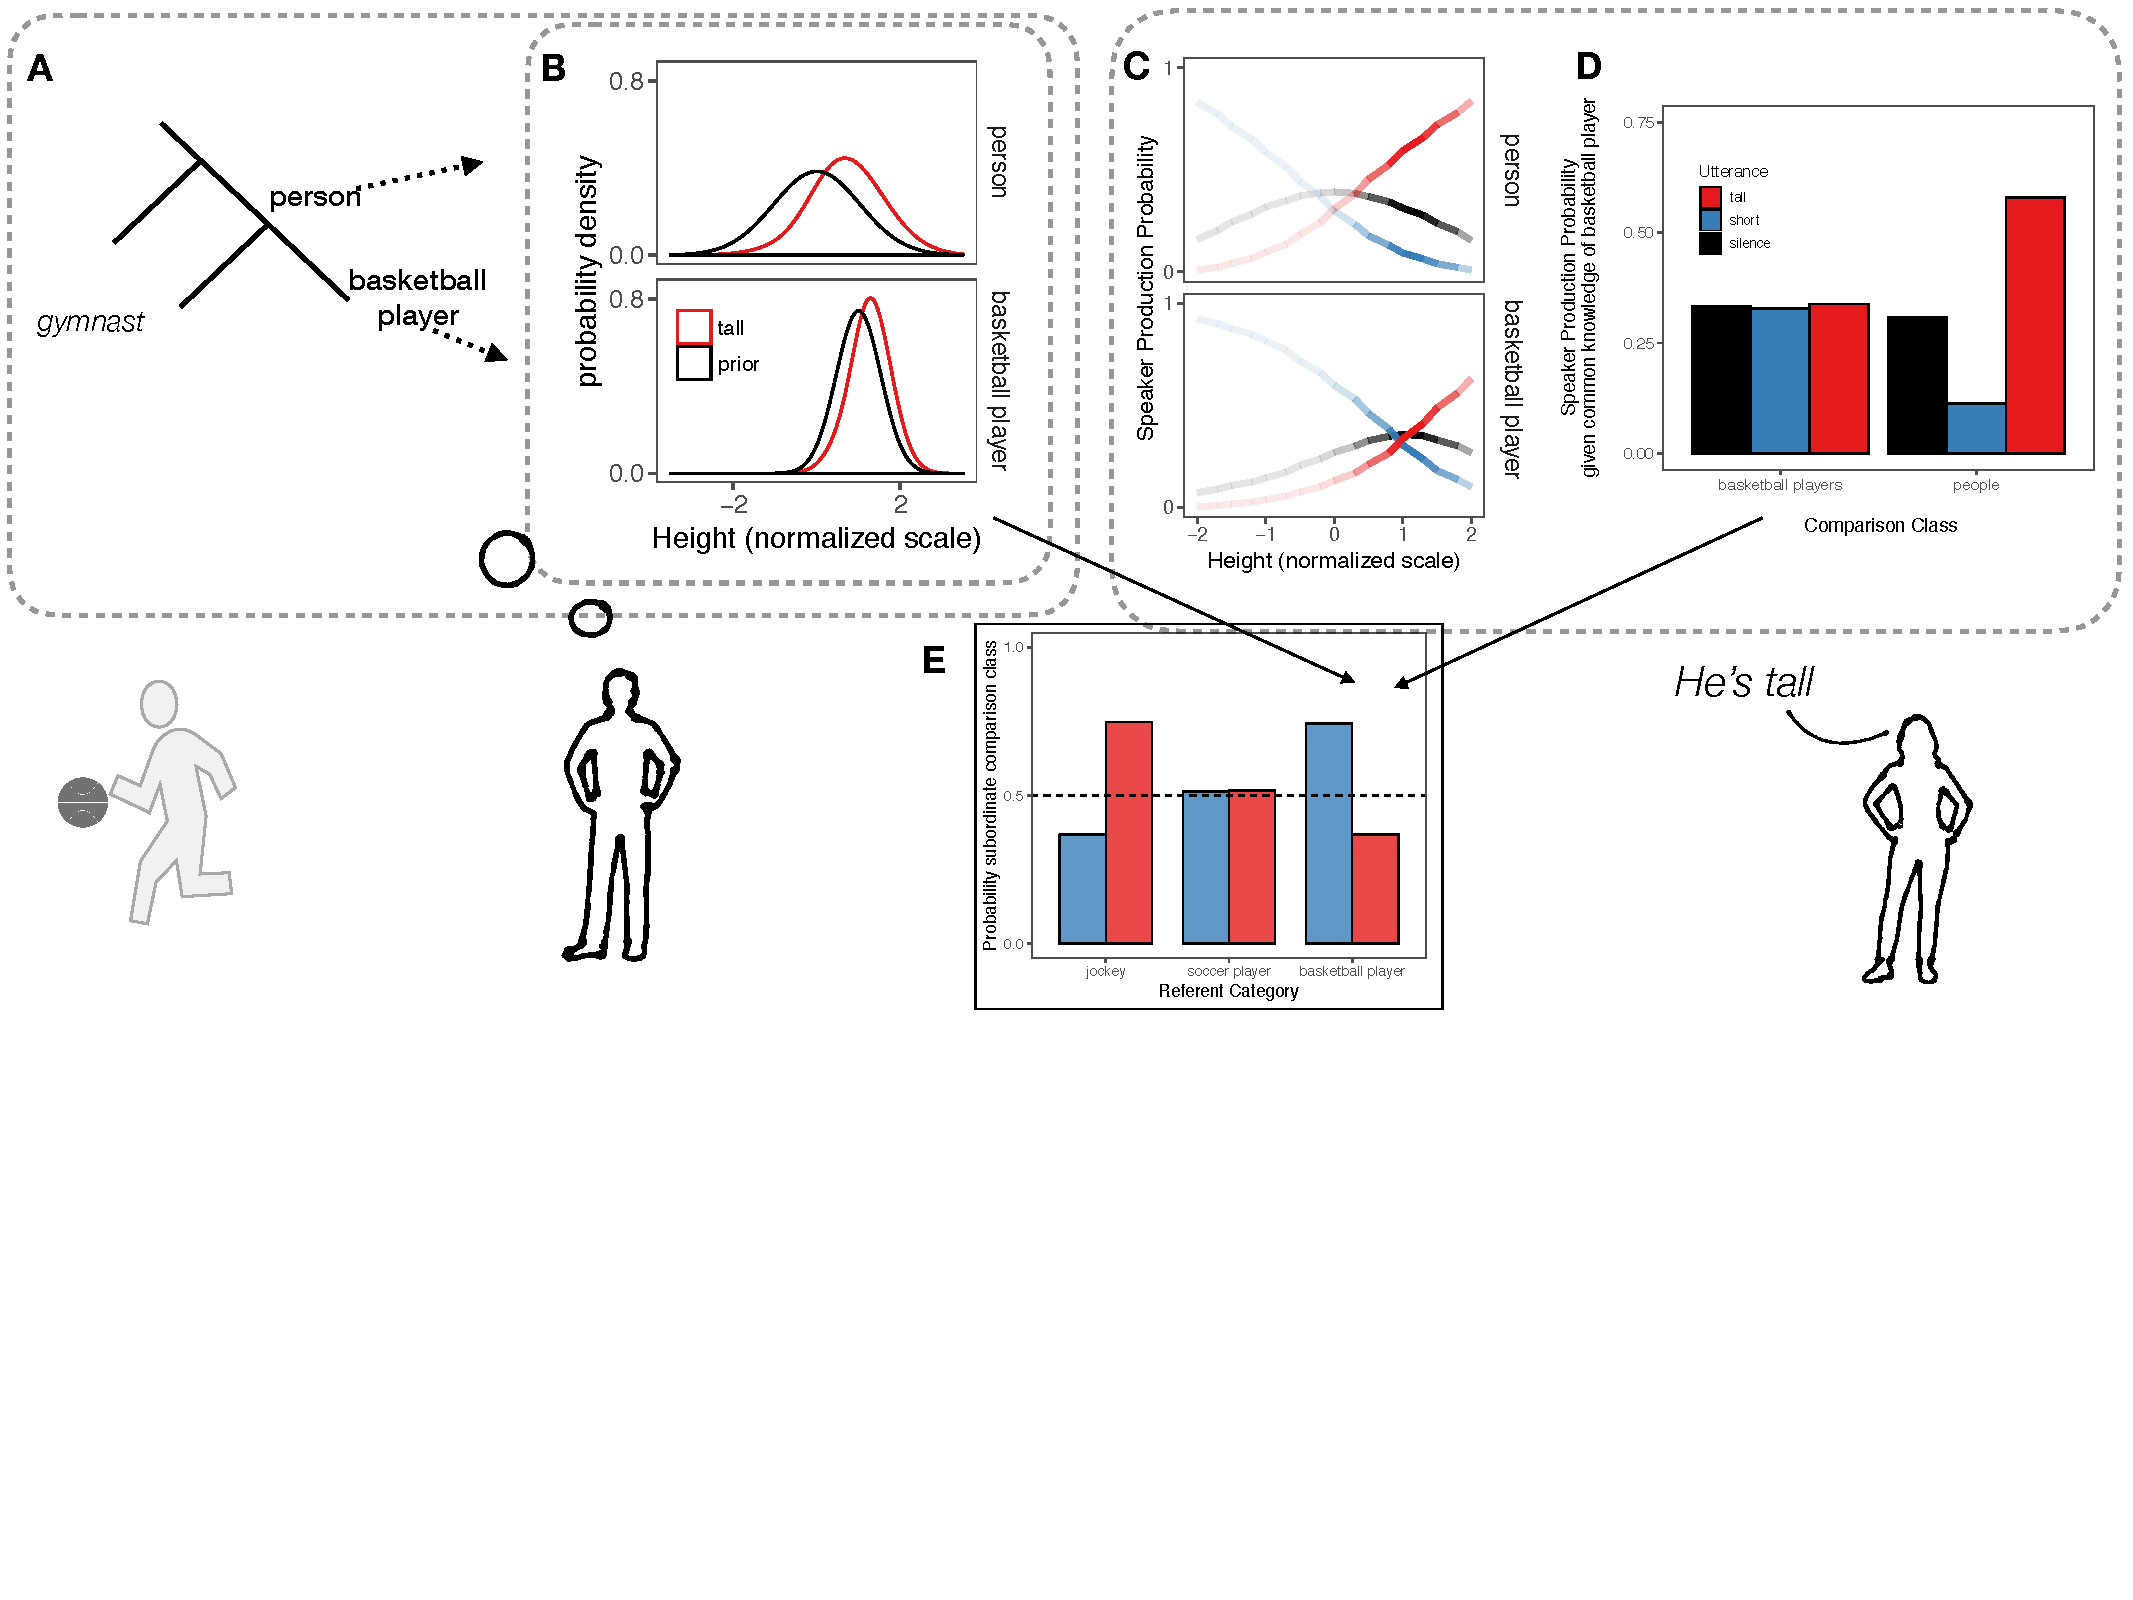
\includegraphics[width=\textwidth]{figs/model_cartoon.pdf}
\caption{\small \label{fig:modelCartoon}Model overview. A listener hears a basketball player described as ``tall'' by a speaker. A: A hypothesis space of comparison classes is constructed over a taxonomic hierarchy. B: A comparison class is realized as a probability distribution over the relevant degree (e.g., height; shown in black). The interpretation of a gradable adjective (e.g., \emph{tall}; shown in red)---given by $L_{0}(x \mid u, c)$---is a function of the comparison class (facets). C: Listener $L_1$ imagines what a speaker $S_1$ would say given different heights of the referent (x-axis) and assuming different comparison classes (facets); the opacity of the colors is in proportion to the listener's prior beliefs of that particular height (e.g., the listener knows the referent is a basketball player, and so expects heights towards the upper range of the scale). D: Speaker utterance production probabilities for different comparison classes, marginalizing over the plausible heights of the referent. A speaker is more likely to say \emph{tall} if the comparison class is \emph{people}. E: Pragmatic listener inferences about the comparison class is computed via Bayes Rule with the utterance likelihood model given by this speaker. Listener is more likely to infer \emph{basketball players} as the comparison class when the referent is described as \emph{short} than when they are described as \emph{tall}. Prior distribution of heights for people is a unit normal distribution $\mathcal{N}(0, 1)$ and the heights of basketball players is a right-shifted normal with smaller variance $\mathcal{N}(0, 0.5)$.
% speaker production probability distributions are shown with the.
}
\end{figure}
  
  
%\subsection{Model behavior}

We consider an idealized case where the comparison class can be either a relatively subordinate-level category ($c_{sub}$) or a relatively superordinate-level category ($c_{super}$) categorization (e.g., tall relative to \emph{basketball players} or relative to \emph{people}): \(c \in \{c_{sub}, c_{super}\}\).
Figure \ref{fig:modelCartoon}C shows the speaker production probabilities of the three possible utterances (\emph{tall}, \emph{short}, silence) for each value along the degree scale (e.g., each height) for each of the two different comparison classes (facets). 
If the comparison class is \emph{basketball players}, the speaker will be reluctant to produce \emph{tall} until the height is substantially greater than average (red line shifted to the right with respect to the \emph{person} comparison class). 
The listener uses Bayes' rule to ``invert'' this generative model of the utterance (i.e., the speaker model), inferring the implicit comparison class.
In doing so, the listener deploys his prior knowledge about the height of the referent: The listener knows the referent is a basketball player and thus their height is distributed according to the basketball player distribution (Figure \ref{fig:modelCartoon}B, bottom, black; this distribution is superimposed as an opacity on Figure \ref{fig:modelCartoon}C).
Averaging over the plausible heights of a basketball player, the listener reasons that a speaker who says \emph{tall} would be more likely to do so assuming the comparison class of \emph{people}  (Figure \ref{fig:modelCartoon}D). 
Thus, the listener who hears \emph{tall} tends to think \emph{tall for a person}, whereas the listener who hears a jockey described as \emph{tall} tends to think \emph{tall for a jockey} (Figure \ref{fig:modelCartoon}E).
Though an intuitive pattern, this reasoning requires a listener separating the comparison class from their own knowledge of the category when reasoning about the meaning of the utterance; an analogous non-pragmatic, literal listener cannot draw this inference (see Supplementary Information).

%To understand the model behavior, consider the speaker model \(S_1\) under different assumptions (by the listener) about the implicit comparison class: \(S_{1}(u \mid x, c = c_{sub})\) and \(S_{1}(u \mid x, c = c_{basic})\). 
%  If the comparison class is \emph{basketball players}, the speaker's criterion shifts to the right and she becomes more reluctant to produce \emph{tall} until the height of the referent is much greater. 

%  If the listener marginalizes out the height of the referent, to focus on the comparison class, they believe the speaker is more likely to produce \emph{tall} if the comparison class were \emph{people} (Figure \ref{fig:modelCartoon}D).  
%If, however, the listener hears of the basketball player that he is \emph{short}, the more likely comparison class is the subordinate class of \emph{basketball players}.
%This inference is driven by prior knowledge about the category, and thus, we would expect the inferences to change if the prior knowledge changes.
%Indeed, the same adjectives used to describe a member of a subordinate category that tends to fall low on the degree scale (e.g., jockeys, who tend to be short people) will result in the opposite inferences about the comparison class (Figure \ref{fig:modelCartoon}E left bars). 
%Thus, our model predicts that the comparison class can be flexibly adjusted and it provides a precise quantitative formulation in how this inference should depend upon the quantitative details of the priors. 

\ndg{this basic pattern is very intuitive, so we should explain a bit more why we need this fancy model. (not sure if that should be here or elsewhere, but i felt it here and at the intro to this section.}

%\begin{figure}
%\centering
%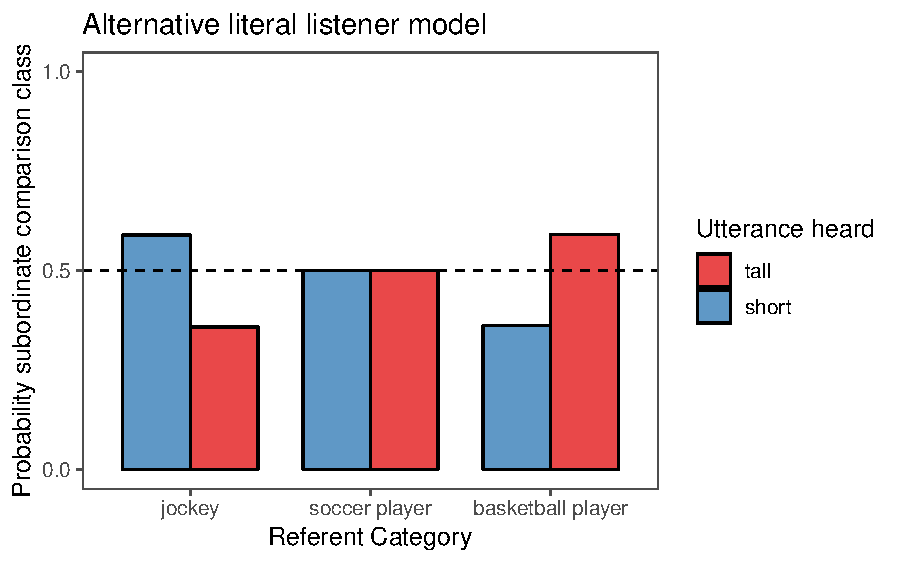
\includegraphics[width=0.6\textwidth]{figs/cc_inference_L0.pdf}
%\caption{\small \label{fig:alternativeModelPredictions}}
%\end{figure}

%The utterance which does not reference a class (e.g., It's warm}) inherits the same meaning as the utterance with the explicit class that
%matches the assumed implicit class (i.e., if \(c_{i} = c_{sub}\), then
%\(u_i\) has the same meaning as \(u_{sub}\)). Therefore, reasoning about
%the likely comparison class reduces to reasoning about which explicit
%utterance the speaker would have been more likely to say.


% it involves representing a speaker's beliefs about the context separately from the listener's beliefs about the context. 
%This can be seen by comparing and \ref{eq:L0}: the pragmatic listener $L_1$ uses a prior distribution over the degree given their knowledge of the referent $P(x \mid k)$ whereas the literal listener $L_0$ uses a distribution conditional on the comparison class $P(x \mid c)$. 
%This separation of the listener's knowledge of the referent $k$ from the comparison class $c$ is necessary for the comparison class inferences shown in Figure \ref{fig:modelCartoon}E.
%A purely Bayesian listener model, who has uncertainty about the comparison class as well as all of the other parameters of the full model (the degree $x$ and the threshold $\theta$), but does not separate their knowledge of the referent from the speaker's representation of the context is given by: 
%  


\section{Behavioral Experiment}

%\section{Overview of Experiment}

We test the model prediction that the comparison class can be flexibly adjusted based on world knowledge and pragmatic principles in a large-scale, web-based free-production experiment.
In the experiment, participants rephrase a speaker's statement which involves a scalar adjective in a way that makes the comparison class explicit.
We measure comparison class inferences using a free-production measure to provide further ecological validity to our measurements of comparison classes: We wish to see if listeners spontaneously adjust their comparison class depending on world knowledge and pragmatic reasoning.
A smaller-scale, forced-choice version of this task was reported in \citeA{tessler2017warm}.%; here, we conduct a free-production version of this task in order test whether the comparison classes are spontaneously inferred by participants.
Additionally, we measure truth judgments for statements involving scalar adjectives and an explicit comparison class as a norming measure of world knowledge that we use in our quantitative modeling (see SI).
%We model both data sets using the same RSA architecture.
Sample size, exclusion criteria, regression analysis, and cognitive model analysis were preregistered for the Comparison Class Inference task: \url{osf.io/xuc96}.

%The quantitative predictions of the model are tested using a joint Bayesian data analytic strategy, where we explicitly model the data from both the Comparison Class Inference and Adjective Endorsement tasks.
%This joint Bayesian data-analytic strategy allows us to infer from simple linguistic judgments the world knowledge that guides the inference about the comparison class in the computational model. 

%\mht{may want to reverse the order, if we use the modal superordinate comparison class from the Inference experiment as the comparison class in the Adjective Endorsement experiment}


 



%To match the  we code the behavioral responses as to whether or not the mention the subordinate level category that is used to describe the referent in the experimental context. 
%
%
%Inferring the comparison class is necessarily a problem of inferring the intentions of another person.
%The relevant question is not \emph{is today a day in winter?} (an inference about the world), but rather \emph{did the speaker mean to draw a comparison to days to winter?} (an inference about intentions).
%Thus, a model for comparison class inference necessarily involves social reasoning about the speaker's intentions.
%
%Thus, the listener's beliefs about the temperature is a probability distribution conditional on the speaker and listener shared beliefs as well as the listener's private beliefs: $P(x \mid f, g)$.
%In the contexts we consider, the listener has no private beliefs and the totality of relevant shared beliefs boils down to the most specific categorization that the listener believes to be true of the referent (i.e., the day is a day in winter).

%On the other hand, on the shared beliefs $g$ can be used to guide 

%
%Both sets of beliefs can constrain the listener's belief distribution over the relevant degree as applied to the referent: If the listener knows that the day is a day in winter, they should use that information to guide their knowledge about the likely value of the degree $P(x \mid f, g)$.
%
%
%We model the scenario where a listener hears a gradable adjective describing a referent (e.g., that the temperature outside is warm) but does not know the comparison class assumed by the speaker. 
%To do this, a listener draws on their knowledge of the referent (e.g., that the day is a day in winter)
%
%When understanding vague language like a gradable adjective in context, a listener must integrate what they know about 
%
%Thus, we begin with a model for gradable adjective interpretation and build a mechanism for comparison class inference on top of this model. 
%. Where does this comparison class come from?
%
%We hypothesize that listeners maintain uncertainty about multiple
%possible comparison classes, but can reduce their uncertainty by
%combining world knowledge with pragmatic reasoning. More specifically,
%listeners use their world knowledge of what worlds are plausible under
%different comparison classes \(P(x \mid c)\) (e.g., the likelihood of
%different temperatures within different seasons), what implicit
%comparison classes are likely to be talked about \emph{a priori}
%\(P(c_i)\) (\(i\) for implicit), and how a rational speaker would behave
%in a given world assuming a particular comparison class
%\(S_{1}(u \mid x, c_i, \theta)\) (Eq. \ref{eq:L1a}). 
%
% As in previous models, we
%assume the listener is aware that the referent is a member of the
%subordinate class (and by extension, the superordinate as well). We
%additionally assume the pragmatic listener uses the most subordinate
%class information to inform the likely values of the degree (e.g., the
%listener's prior over temperatures is given by the distribution of
%temperatures for a specific class such as \emph{winter}
%\(P(x \mid c = c_{sub})\)). With these assumptions, the model becomes:
%
%\begin{align}
%L_{1}(x, c_{i}, \theta \mid u) &\propto S_{1}(u \mid x, c, \theta) \cdot P(x \mid c =  c_{sub}) \cdot P(c_{i}) \cdot P(\theta) \label{eq:L1a}\\
%S_{1}(u \mid x, c_i, \theta) &\propto \exp{(\alpha_1 \cdot \ln {L_{0}(x \mid u, c_i, \theta)}- \text{cost}(u)) } \label{eq:S1a}\\
%L_{0}(x \mid u, c_i, \theta) &\propto {\delta_{[\![u]\!](x, \theta)} \cdot P(x \mid \text{parseClass}(u, c_i))} \label{eq:L0a}
%\end{align}
%
%We are interested in the behavior of the pragmatic listener model with
%he hears an utterance without an explicit comparison class \(u_{i}\)
%(e.g., ``It's warm''). The listener reasons about alternative
%utterances the speaker could have said in order to draw pragmatic
%inferences. In this model, we assume the speaker has the option of
%conveying the adjective with an explicit comparison class \(u_{sub}\)
%and \(u_{super}\) (e.g., ``It's warm relative to other days in
%winter'' and ``It's warm relative to other days of the year'').
%The literal meanings of these alternatives are the same as the
%underspecified utterance (i.e., a threshold function:
%\([\![u_{warm}]\!] = x > \theta\)), but have the additional feature of
%overriding the implicit comparison class \(c_i\)and forcing the literal
%listener into a particular comparison class encoded in the utterance via
%the function \(\text{parseClass}\). That is:
%
%\begin{eqnarray}
%\text{parseClass}(u, c_i) & = &
%\begin{cases}
%c_{i} & \text{if } u = u_{i}\\
%c_{sub} & \text{if } u = u_{sub}\\
%c_{super} & \text{if } u = u_{super}\\
%\end{cases}
%\end{eqnarray}
%
%Thus, the speaker conditioning on a particular value for \(c_{i}\) only
%has implications for the literal listener if the speaker chooses to
%produce the implicit utterance (e.g., ``It's warm''). Should the
%speaker instead choose an utterance that explicitly articulates the
%comparison class (e.g., ``It's warm for winter''), the literal
%listener will use the explicit class to set his prior expectations
%\(P(x \mid c)\) via the \(\text{parseClass}\) operator.
%




%\subsubsection{Qualitative model predictions}


%\begin{figure*}[htb]

%{\centering 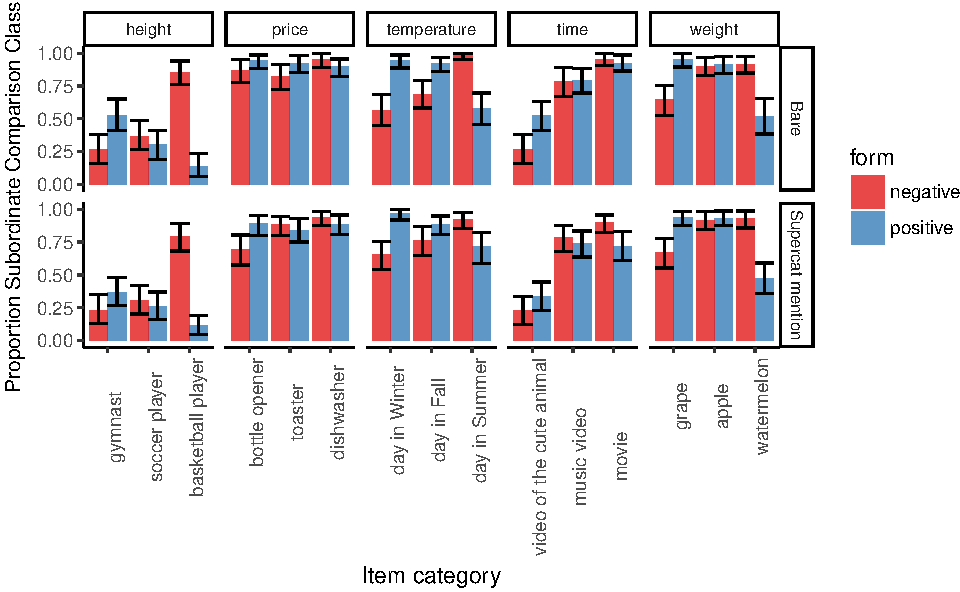
\includegraphics[width=1\textwidth]{figs/expt1results-1} 
%
%}
%
%\caption{Empirical comparison class judgments in terms of proportion in favor of subordinate comparison class.  Error bars correspond to 95\% Bayesian credible intervals.}\label{fig:expt1results}
%\end{figure*}
%
%\begin{figure*}[htb]
%
%{\centering \includegraphics[width=1\textwidth]{figs/modelParameters-1} 
%
%}

%\caption{Reconstructed degree priors (top) and empirically derived comparison class priors (botton). Top: Inferred prior distributions of world knowledge used to model Experiment 1 and 2 data. Bottom: Inferred prior probability of the subordinate comparison classes based on Google WebGram frequencies. Error bars correspond to 95\% Bayesian credible intervals, derived from the posterior on the $\beta$ scale parameter.}\label{fig:modelParameters}
%\end{figure*}





%\subsection{Task 2: Comparison class inference}

%We report detailed methods for Task 2 (Comparison Class Inference) here. 
%Methods and results concerning Task 1 (Stimuli Generation) and Task 3 (Adjective Endorsement) are described in brief here, and in full detail in the Supplement.



\subsection{Methods}

\subsubsection{Participants}

We recruited 837 participants from Amazon's Mechanical Turk. 
This number was arrived at with the goal of estimating the probability of a subordinate~vs.~superordinate comparison class with confidence intervals no larger than 0.20 for each unique item in the data set, which conservatively produced an estimate of roughly 50 responses per item.

Participants were restricted to those with U.S. IP addresses with at least a 95\% work approval rating. 
In addition, participants were required to pass a simple language comprehension test that we designed in order to weed out bots and other bad-faith participants (see SI). 
Participants who fail this check are required to exit the experiment before completing the task, and so we do not have an estimate for how many participants fail this check. 

\red{describe other exclusion criteria}

\subsubsection{Materials}

The experiment involved the interpretation of gradable adjectives that describe physical dimensions (15 pairs in total, e.g., \emph{tall}/\emph{short}; \emph{warm}/\emph{cold}; see Table \ref{tab:1} for full list). 
The categories used in the experiment were a modified subset of a set of adjective-noun pairs generated by a separate group of participants ($n=50$) in a task designed to elicit stimuli for this experiment (see SI for details). 
From this set of participant-generated stimuli, we curated 90 item sets -- (X, Y, Z)  triples -- whose categories were at the same level of abstraction  (e.g., they were all subordinate categories of the same basic-level category) and that made sense in the kinds of minimal contexts we use in the Comparison Class Inference experiment.
Two examples from each adjective pair are shown in Table \ref{tab:1}. 
\ndg{it's confusing to have task 1 materials and methods embedded here in the task 2 methods section. have a small section above instead?}
\mht{moved task 1 details to supplement. okay?}

Each of the 90 item sets contains 3 relatively subordinate categories, which vary in their general expectations (low, medium, high) about some degree (e.g., height), within the same relatively superordinate category (e.g., basketball player [high], soccer player [medium], jockey [low]; superordinate: people).\footnote{
We refer to the level of abstraction of these categories as \emph{relatively} subordinate or superordinate, because the item sets may be sets of (i) subordinate-level categories within the same basic-level category (e.g., Great Danes, chihuahuas, within dogs) or (ii) basic-level categories within the same superordinate-level category (e.g., elephants, squirrels, within animals). Later, we will explicitly model the precise level of abstraction of these categories.
}
The categories within each item set are paired with either a positive-form or negative-form adjective (e.g., tall or short). 
Thus, this experiment had 270 unique categories (90 sets $\times$ 3 levels of general expectations) described with 2 adjectives each (e.g., tall and short), for a total of 540 unique items.


\begin{table*}[ht]
\centering
\begingroup\fontsize{10pt}{11pt}\selectfont
\begin{tabularx}{\textwidth}{lll}
  \hline
Adjectives (scale) & Example subordinate classes (superordinate class) \\ 
  \hline
  \emph{big}, \emph{small} (size) & \emph{great dane}, \emph{poodle}, \emph{chihuahua} (dogs) \\ 
						 & \emph{elephant}, \emph{monkey}, \emph{mouse} (animals) \\ 
\emph{tall}, \emph{short} (height) &  \emph{basketball player}, \emph{golfer}, \emph{jockey} (people) \\ 
							&  \emph{redwood}, \emph{alpine}, \emph{bonsai} (trees) \\ 
  \emph{expensive}, \emph{cheap} (price) & \emph{boots}, \emph{sneakers}, \emph{sandals} (footwear) \\ 
						   & \emph{steakhouse}, \emph{buffet}, \emph{diner} (restaurants) \\ 
    \emph{warm}, \emph{cold} (temperature) & \emph{summer}, \emph{fall}, \emph{winter} (seasons) \\ 
							& \emph{soup}, \emph{salad}, \emph{ice cream} (food) \\ 
    \emph{hot}, \emph{cold} (temperature) & \emph{coffee}, \emph{juice}, \emph{milkshake} (drinks) \\ 
								& \emph{sauna}, \emph{shopping mall}, \emph{ice rink} (places) \\ 
  \emph{heavy}, \emph{light} (weight) &  \emph{wool}, \emph{cotton}, \emph{silk} (materials) \\ 
							  &  \emph{rock}, \emph{stick}, \emph{feather} (objects) \\ 
  \emph{long}, \emph{short} (duration / length) & \emph{slacks}, \emph{capris}, \emph{shorts} (pants) \\ 
								  & \emph{novel}, \emph{story}, \emph{poem} (readings) \\ 
  \emph{loud}, \emph{quiet} (loudness) &   \emph{baby}, \emph{teenager}, \emph{adult} (people) \\ 
							  &  \emph{auditorium}, \emph{classroom},   \emph{study hall} (rooms) \\ 
 \emph{noisy}, \emph{quiet} (loudness) &  \emph{horn}, \emph{guitar}, \emph{harp} (instruments) \\  
							 &  \emph{powerboat}, \emph{sailboat}, \emph{row boat}  (boats) \\  
  \emph{light}, \emph{dark} (luminance) & \emph{day}, \emph{dusk}, \emph{night}  (times of day) \\  
								  & \emph{white paint}, \emph{blue paint}, \emph{black paint}  (paints) \\  
   \emph{fast}, \emph{slow} (speed)   &  \emph{runner}, \emph{skier}, \emph{weight lifter} (athletes) \\
								  &  \emph{glider}, \emph{helicopter}, \emph{plane} (aircraft) \\
  \emph{quick}, \emph{slow} (speed) &  \emph{rabbit}, \emph{cat}, \emph{turtle} (pets) \\
							  &  \emph{instant pot}, \emph{frying pan}, \emph{crockpot} (cookware) \\
  \emph{strong}, \emph{weak} (strength) &  \emph{hurricane}, \emph{thunderstorm}, \emph{rain} (storms)\\
						  &  \emph{lion}, \emph{dog}, \emph{mouse} (animals)\\
  \emph{hard}, \emph{soft} (hardness) &  \emph{jolly rancher}, \emph{chocolate}, \emph{marshmallow} (sweets)\\
							  &  \emph{tile}, \emph{wood}, \emph{carpet} (floor materials)\\
  \emph{wide}, \emph{narrow} (width) & \emph{boulevard}, \emph{street}, \emph{country lane} (roads) \\
							  & \emph{truck}, \emph{car}, \emph{golf cart} (vehicles) \\
   \hline
\end{tabularx}
\caption{Example sets of adjectives and categories used in Experiments 2 and 3. 
Categories were curated from a set of empirically elicited noun phrases (Experiment 1).} 
\label{tab:1}
\endgroup
\end{table*}



\subsubsection{Procedure}

%Following the language comprehension test (described above), participants read instructions about the task. 
In a warm-up trial, participants were told they they would be asked to rephrase something a person said:  the person said a word that is relative and their task was to figure out what the word was relative to. They were given the example of \emph{John says: ``The Empire State Building is tall''} and asked to fill-in a sentence with the same kind of response they would do on the main trials (i.e., \emph{The Empire State Building is tall relative to other \_\_\_}). Participants were told to fill in the blank with a group or category that makes the most sense and to use their common sense.
Responses to this warm-up trial were used as a basis for exclusion (any response other than buildings, structures, towers, skyscrapers, etc.). 

%On each trial, participants were given a context sentence to introduce
%the subordinate category (e.g., \emph{Tanya lives in Maryland and
%steps outside in winter}). This was followed by an adjective sentence, which predicated either a positive- or negative-form gradable adjective over the item (e.g., \emph{Tanya says to her friend, ``It's warm.''}). Participants were asked \emph{What do you think Tanya meant?} and given a sentence frame they could complete with with a freely-produced comparison class:

Participants then completed 36 main trials. Each main trial began with a \emph{context sentence} that introduced the referent as a member of a subordinate category and provided an appropriate but minimal context in which the adjective could be uttered (e.g., \emph{John sees a \{basketball player, golfer, jockey\}}); the same context sentence was used for all 3 categories in an item set.
Then, a speaker utters an adjectival utterance predicating the adjective of a pronoun used to refer to the referent (e.g., \emph{John says: ``They're tall''}).\footnote{
We had the speaker use a pronoun so as to not provide a strong linguistic cue as to the intended comparison class. If the referent was a person, we used  the singular ``they'' to refer to them; otherwise, we used either ``it'' or ``they'' depending on the plurality of the referent. 
}
The participant was asked what they thought the speaker meant (e.g., \emph{What do you think John meant?}). Participants responded by freely filling in a sentence that required an explicit comparison class: 

\begin{quote}
They're tall relative to other \_\_\_\_\_\_.
\end{quote}

We used the word ``other'' to invoke the presupposition that the referent is a member of the comparison class. Pilot testing suggesting that omitting this word invoked many direct comparisons to singular entities (e.g., \emph{They're tall relative to their short friend}), which were wildly heterogeneous in nature. 

At the end of the task, participants were asked a memory check question where they had to select, from a list of 10 options, all of the items they could recall seeing. In the memory check, items were shown as adjective -- noun pairs (``tall -- basketball player'') and the 5 distractors were either color or multidimensional adjectives paired with a category that was not used in our test stimuli (e.g., ``green -- tennis ball''; ``beautiful -- painting'').
This memory check trial was also used as a basis for exclusion. 

\begin{figure}[t!]
\centering
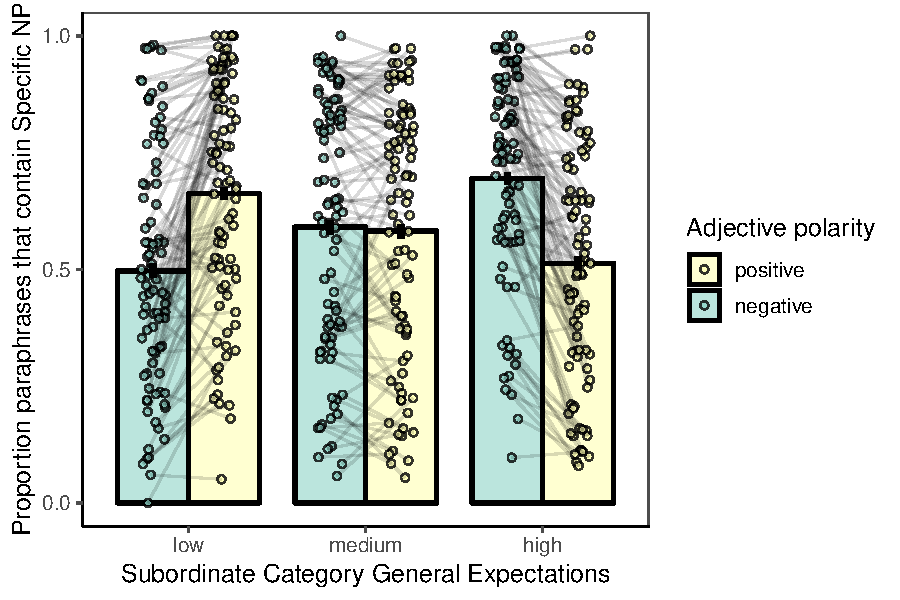
\includegraphics[width=0.7\textwidth]{figs/bars_cc_finalExpt_prereg_bars_syncDodge.pdf}
%{\centering 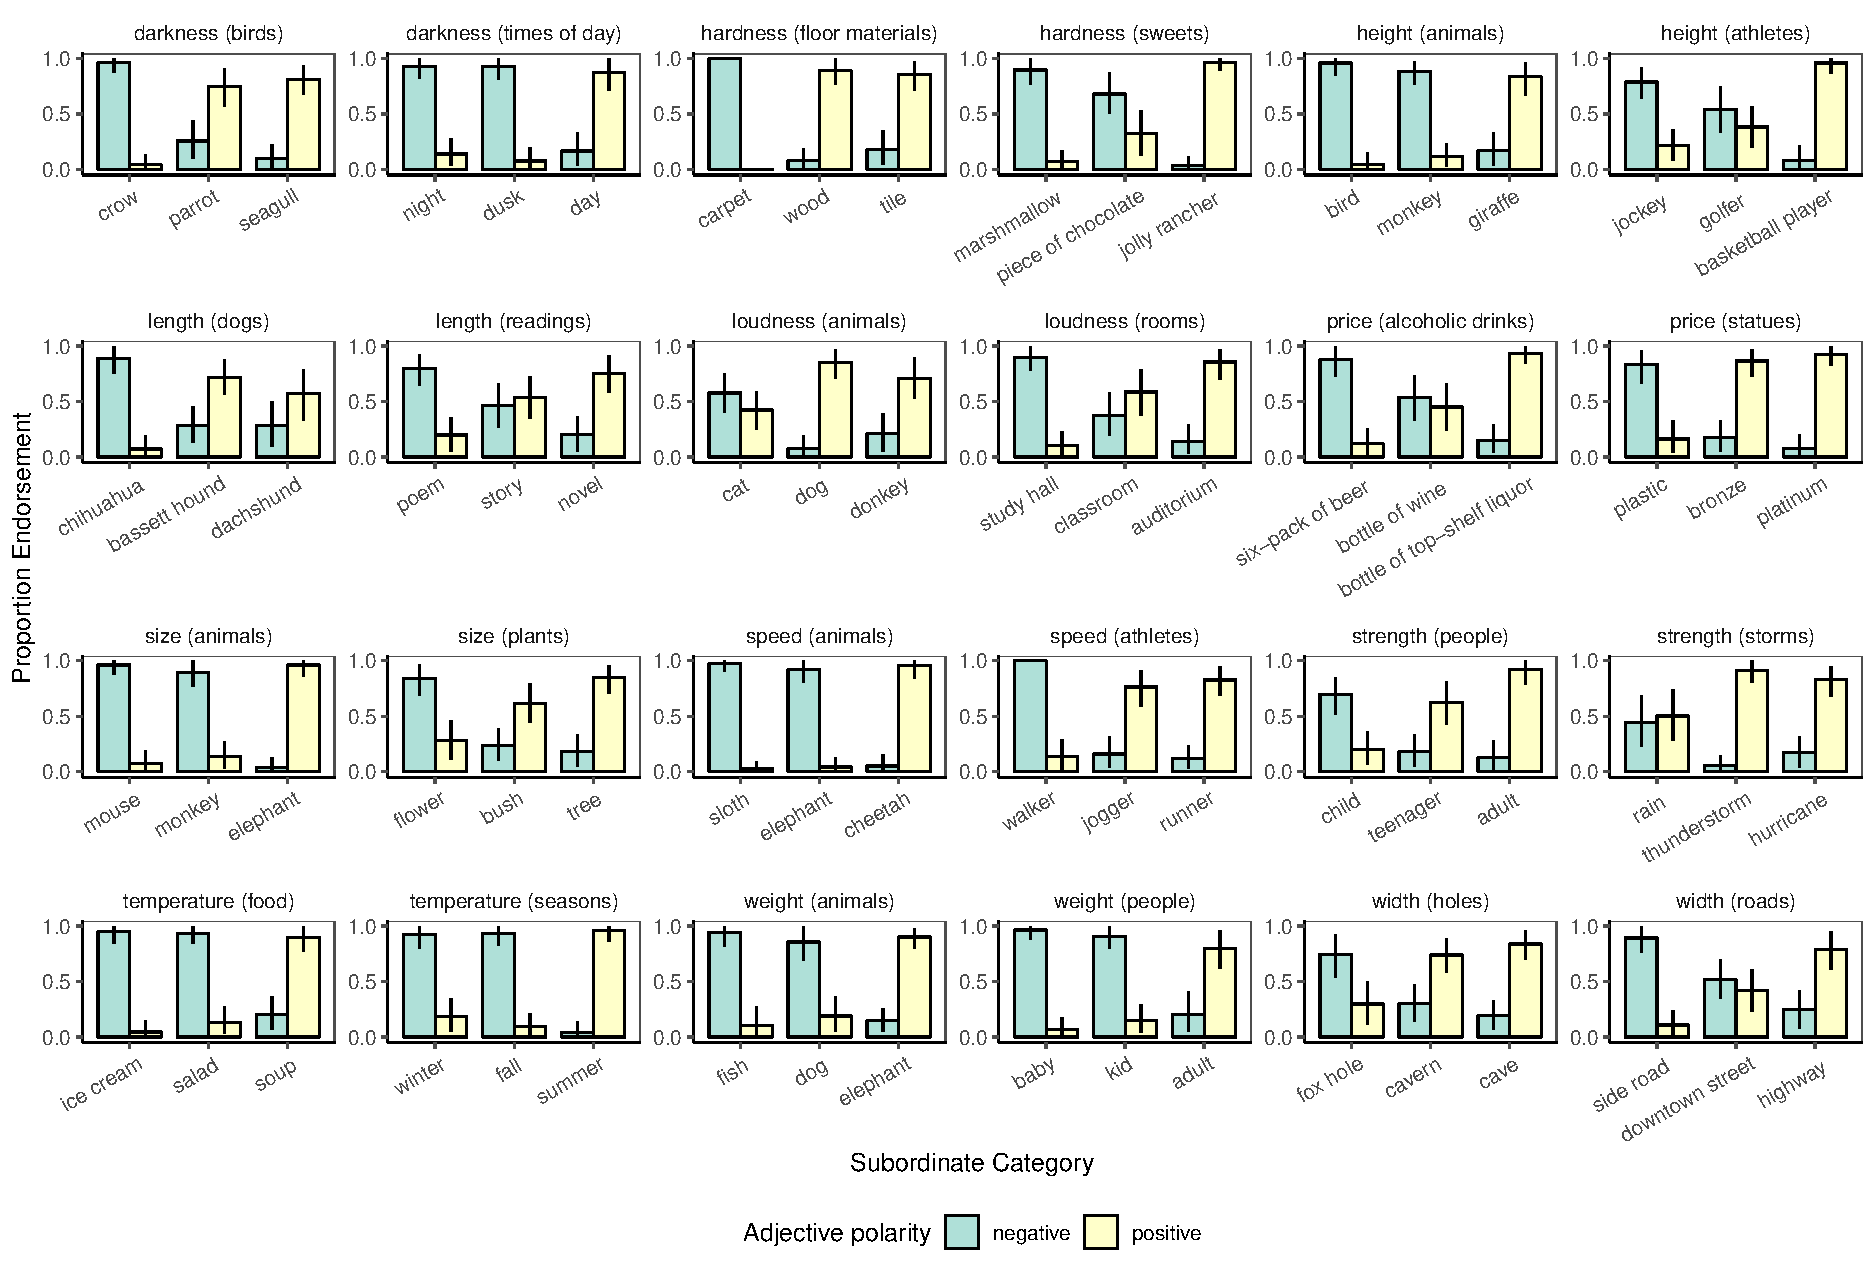
\includegraphics{figs/bars_adj_finalExpt_pilot_byItem} }
\caption{Comparison Class Inference experimental results. Proportion of paraphrases that contained the Subordinate NPs (e.g., \emph{basketball player}) with which the referent was introduced, as a function of the general expectations listeners have about the category (x-axis) and the polarity of the adjective used to describe the category (e.g., \emph{tall} = positive, \emph{short} = negative). Bars represent overall means and error bar is a bootstrapped 95\% confidence interval. Each dot represents the mean of a single item and lines connect Subordinate NPs described with different adjectives (e.g., \emph{tall} and \emph{short} basketball player). Dots are jittered horizontally to improve visual clarity.}\label{fig:ccInferenceItems}
\end{figure}

\subsection{Results}

Participants were excluded if they either responded incorrectly to the warm-up trial (answering something other than \emph{buildings}, \emph{skyscrapers}, \emph{structures} or the like) or answered fewer than 7 out of 10 memory check questions accurately.\footnote{Incorrect responses to the warm-up trial were most often indicative of copying some part of the text on the screen and pasting it into the response box (e.g., responding with the name of the speaker, just putting the adjective ``tall'', or responding with a whole sentence without a comparison class ``that is tall'').}
750 participants (89.6\%) remained after these exclusion criteria, for a total of 27,000 responses.
We additionally excluded nonsensical responses: these were primarily responses that just listed the name of the speaker, the adjective alone, or restated the full adjectival sentence (e.g., ``It is tall'') and numbered 420 (1.56\%) in total, leaving 26,580 codeable responses. 
We processed the responses by correcting for misspellings, lemmatizing, and collapsing across synonyms. 

\subsubsection{Preprocessing}

In order to improve alignment across responses, we corrected for misspellings (569; 2.14\%), lemmatized to align plural and singular responses (e.g., \emph{baby} and \emph{babies}; 867, 3.28\%), and replaced some responses with obvious synonyms (e.g., \emph{child}--\emph{kid}; \emph{booze}--\emph{alcoholic drink}; \emph{humans}--\emph{people}; 323, 1.22\%). 

Pilot testing suggested that participants primarily provide comparison class paraphrases that are identical to the subordinate noun phrase by which the referent is introduced (\emph{subordinate-NP}, e.g., a basketball player) or a more superordinate category (\emph{superordinate-NP}). 
We automatically categorize responses as either subordinate or superordinate by checking whether the preprocessed response contains the subordinate-NP or superordinate-NP\footnote{Some of our pre-designated superordinate-NPs turned out to be incorrect guesses as to what would be the most salient superordinate category in the context. These cases were all very clear, and we replaced our pre-designated superordinate-NPs with the empirical superordinate-NP for purposes of analysis.} as a substring, respectively. \footnote{This analysis assumes that in order to convey a category at least as specific as the subordinate-NP, one must include the subordinate-NP in the response. 
For example, \emph{male basketball players} is more specific than \emph{basketball players} and includes the substring \emph{basketball player}. Negation markers (e.g., ``all kinds of people except basketball players'') are one case where this assumption would be invalid, but no responses contained any.}
22161 (83.4\%) of valid responses could be automatically categorized as either the subordinate-NP or a superordinate-NP that was consistent across items in the item set. 
%\red{For example, in response to  \{basketball players, golfers, jockeys\} are \{tall, short\}, \textbf{X\%} of participants produced either one of the three specific NPs or the more general \emph{people}}. \mht{[how common is athlete here?]}
We use only these data for the main analyses.
Of the remaining 4394 (16.6\%) responses, 1966 were unique.
We hand-annotated these remaining responses; the main results and conclusions are consistent when analyzing the full data set (see SI).




\subsubsection{Regression analysis}
Our primary hypothesis was that usage of a subordinate~vs.~superordinate comparison class would be influenced via an interaction between the general expectations about the category and the polarity of the adjective (Figure \ref{fig:ccInferenceItems}), which we tested with a maximal Bayesian mixed-effects model.\footnote{
	For the regression analysis, we predict subrodinate-NP paraphrases as a function of the general expectations about the subordinate category (low, medium, high; dummy coded with the medium category as the reference level), the adjective (positive vs. negative; difference coded), and their interaction; in addition, we include the maximal mixed effects structure by-item set and by-participant that mirrors this fixed effects structure. The model is subordinate\_inference $\sim$ gen\_expectations * adjective\_polarity + (1 + gen\_expectations * adjective\_polarity | participant) + (1 + gen\_expectations * adjective\_polarity | item\_set).
} 
%As predicted by the comparison class inference model, listener inferences about the comparison class were influenced via an interaction between the general expectations about the subordinate category and the adjective polarity , which 
%We confirmed 
%Our comparison class inference model makes qualitative predictions about the likely comparison class assumed by a speaker when they hear a scalar adjective (e.g., \emph{he's tall}; Figure \ref{fig:modelCartoon}E).
We observe an overall preference for subordinate comparison classes for the control (middle-of-the-scale) subordinate categories (e.g., \emph{soccer players}; \brmresults{expt3_brm_pilot.csv}{Intercept}) and no credible difference in this overall preference when the subordinate category was either near the high-end of the scale (e.g., \emph{basketball players}; \brmresults{expt3_brm_pilot.csv}{np_expectationshigh}) or the low-end of the scale (e.g., \emph{gymnasts}; \brmresults{expt3_brm_pilot.csv}{np_expectationslow}).
 In addition, there was no credible difference in comparison class inferences for the positive form adjective (e.g., tall) and the negative form adjective (e.g., short) for the middle-of-the-scale, control items (e.g., \emph{soccer players}; \brmresults{expt3_brm_pilot.csv}{adj_polarity1}.

As predicted by the comparison class inference model, we observe a pair of two-way interactions:
When the subordinate category was expected to be near the high-end of the scale (e.g., basketball player), the negative-form adjective (e.g., short) led to more subordinate comparison classes than the positive-form adjective (e.g., tall) in comparison to the control, middle-of-the-scale items (e.g., soccer player):  beta-weight and 95\% Bayesian credible interval: \brmresults{expt3_brm_pilot.csv}{np_expectationshigh:adj_polarity1}.
The opposite interaction was observed for categories that were expected to be near the low-end of the scale (e.g., gymnast player): Hearing the positive-form adjective led to credibly more subordinate inferences than hearing a negative-form adjective, in comparison to the middle-of-the-scale subordinate categories:  \brmresults{expt3_brm_pilot.csv}{np_expectationslow:adj_polarity1}.
Thus, general, world-knowledge expectations about the category interface with the adjective used to predicate the referent to guide comparison class inferences, as predicted by the model.


\begin{figure}[t!]
\centering
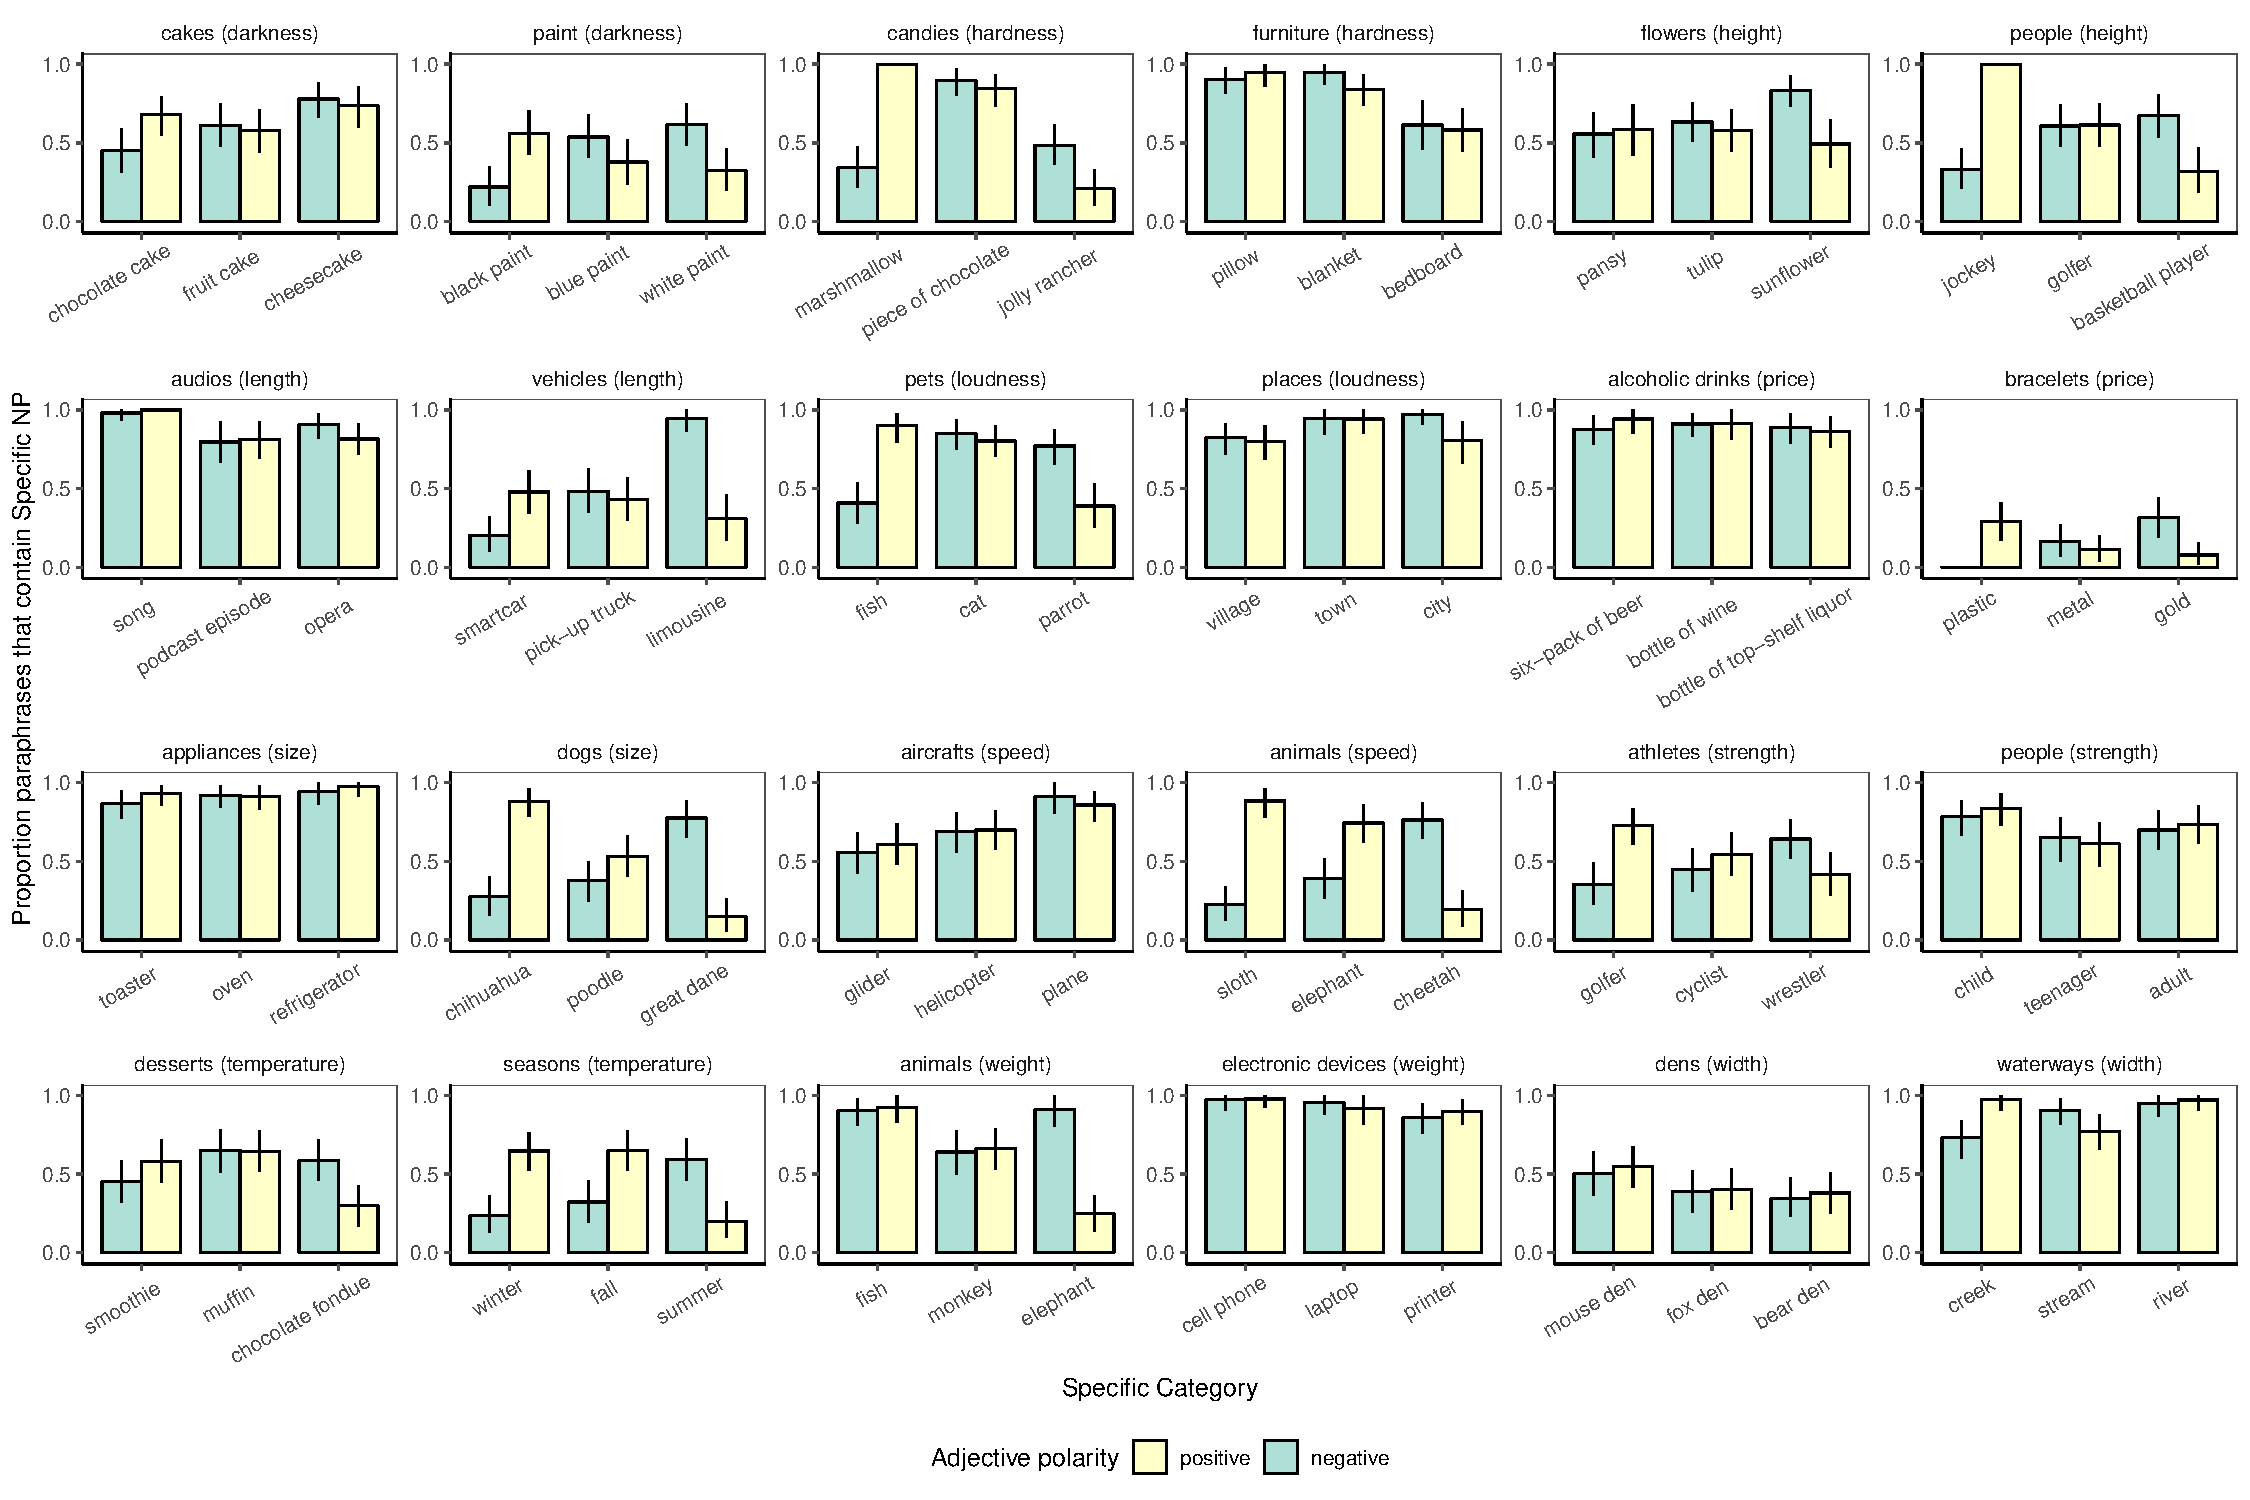
\includegraphics[width=\textwidth]{figs/bars_cc_finalExpt_prereg_byItem.pdf}
%{\centering 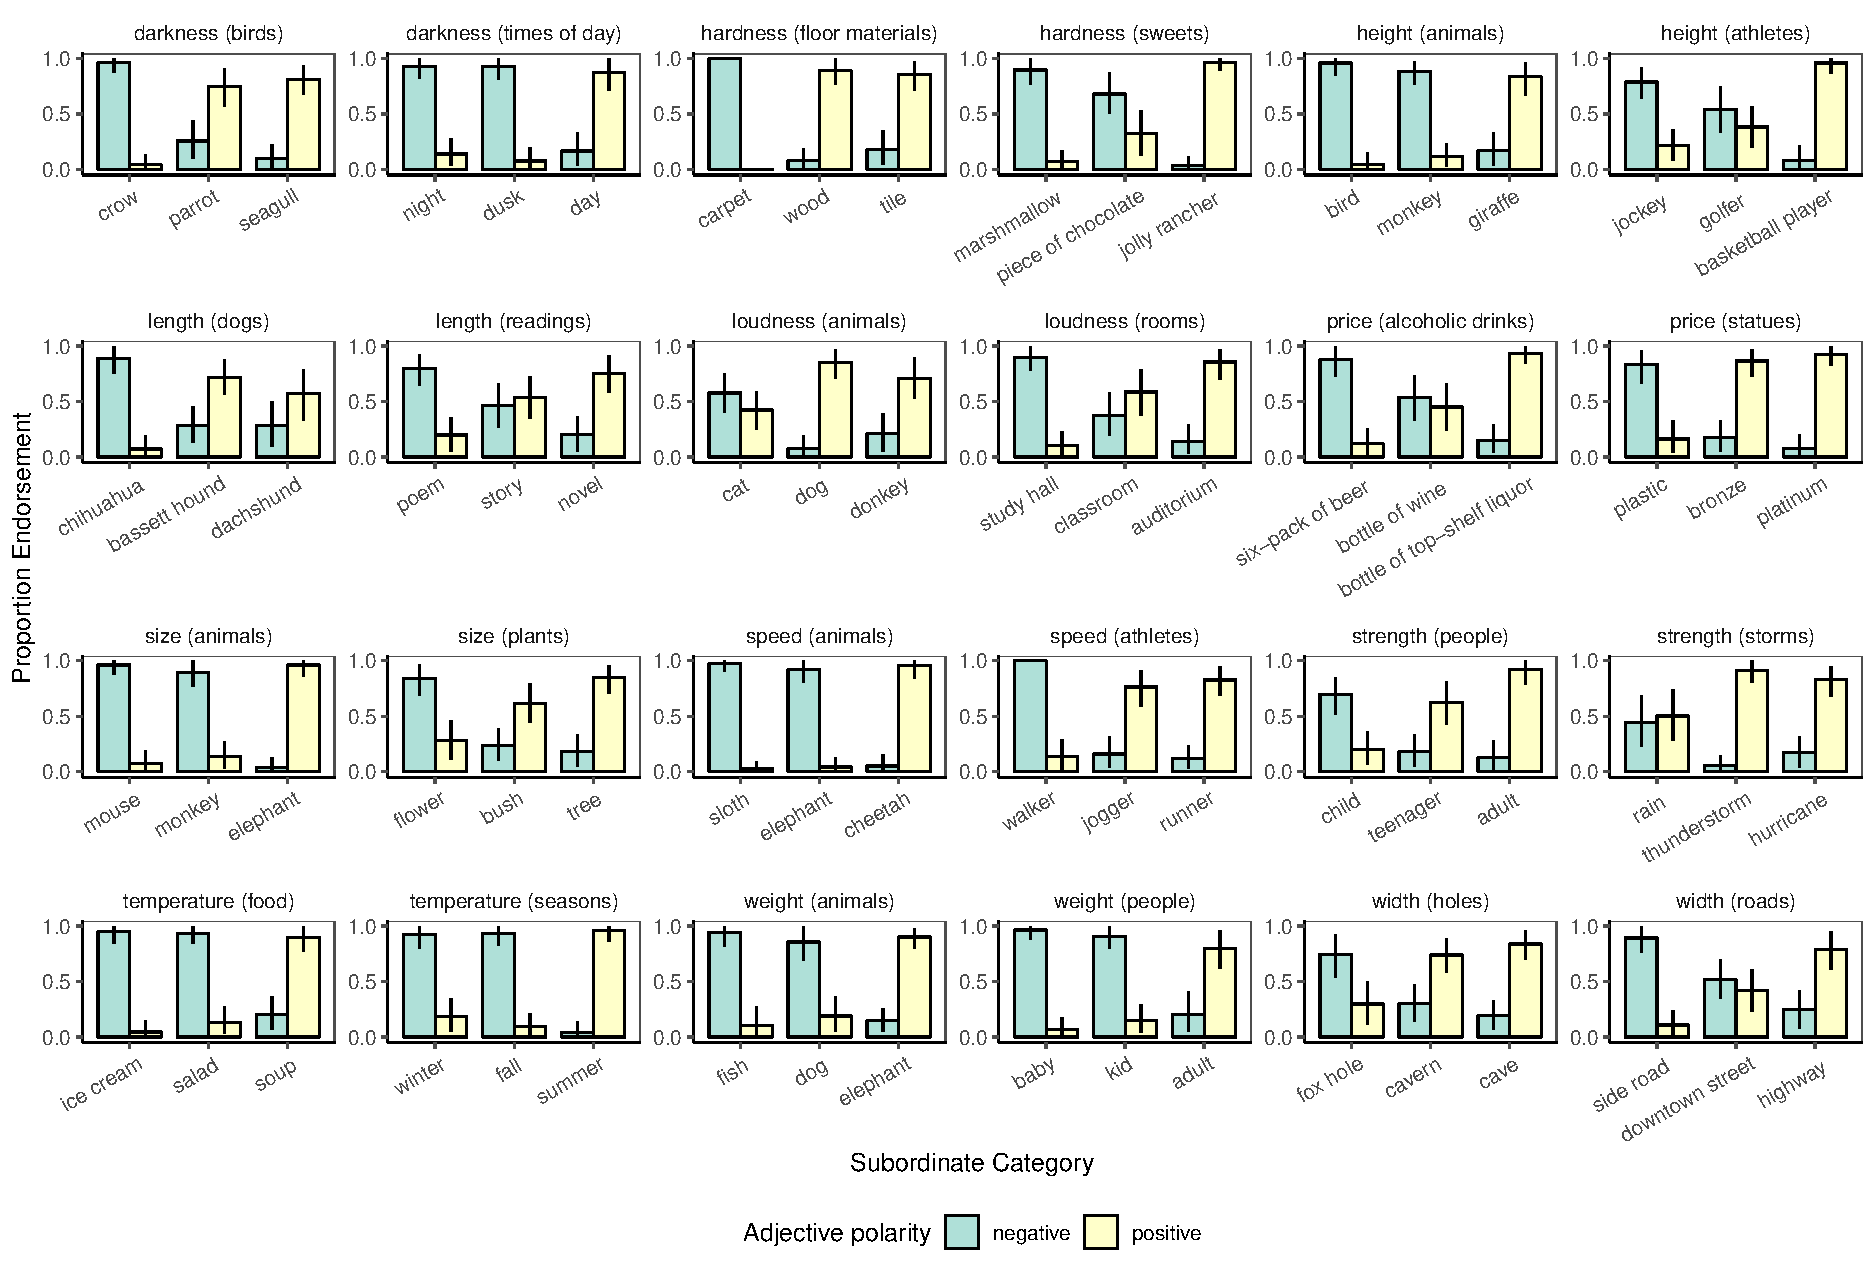
\includegraphics{figs/bars_adj_finalExpt_pilot_byItem} }
\caption{Comparison class inference results for 24 of the 90 items. Two examples were selected from each unique degree scale; example items were those that exhibited the greatest and smallest variability in comparison class inferences.}\label{fig:ccInferenceItems}
\end{figure}





%is analysis confirms the primary hypothesis.
\ndg{these results are hard to understand. partly because the terms are hard to process (specific, subordinate, etc), also because you jump into the most complex analysis. maybe lay it out like a standard behavioral analysis, describing the regression model and then walking through main effects before interactions? then say connection to model...}
\mht{any better?}


The overall preference for a subordinate level comparison class and the magnitude of the effect of the adjective-predicated varies considerably by item (Figure \ref{fig:ccInferenceItems}).
We turn to the quantitative aspect of our model to triangulate the sources of variability that give rise to these item-wise differences.

\subsection{Quantitative modeling of item-variability}

%We then test the simple effects. For items low on the degree scale (e.g., temperatures in winter), positive form adjectives were significantly more likely to imply subordinate comparison classes (\(\beta = 1.41\); \(SE = 0.15;\) \(z = 9.43\)), while the opposite is true for items high on the scale (e.g., summer days; \(\beta = -2.50\); \(SE = 0.19;\) \(z = -13.15\)). Participants reason pragmatically to flexibly adjust the comparison class, combining world knowledge with informativity as predicted by our model.

Our model is not only useful for understanding the basic computations that underly comparison class inference, it is a tool for characterizing the subtleties of comparison class inference by way of the gradience in the model's predictions.
The model's primary capacity to predict gradience in comparison class inference is as a function of distributional knowledge about scalar properties of categories $P(x)$ (e.g., the heights of basketball players, temperatures in Winter, ...), or what we've been calling \emph{general expectations} about the category.
Variance in inferences that cannot be explained by world knowledge can be captured in the model via the comparison class prior $P(c \mid k$), which encodes baseline expectations about the comparison class given the category membership of the referent.
Baseline expectations about conceptual comparison classes could be a function of the level of abstraction of the categories in question \cite<e.g., exhibiting a basic-level bias;>{rosch1975family} as well as the usage frequency of the NPs used to describe those categories. 
We thus construct a family of alternative models in order to gain insight into the sources of variability in comparison class inferences; these models differ in their parameterization of the comparison class prior: (1) a ``flat prior model'', which assumes the comparison class prior assigns equal probability between subordinate and superordinate classes; (2) an ``intercept only'' model, which assumes a basic-level bias, (3) a ``slope only'' model, which assumes an effect of usage frequency, but no basic-level bias, (4) a ``slope and intercept'' model, which assumes both a basic-level bias and an effect of usage frequency.\footnote{
Because our stimuli were largely generated by a separate group of participants,  we do not know \emph{a priori} if the NPs we use to introduce the referents in the task are basic-level categories or subordinate level categories, and hence, whether the more superordinate comparison class would correspond to a superordinate-level category or a basic-level category.
A basic-level bias could plausibly operate differently for a subordinate~vs.~basic-level inference than for a basic~vs.~superordinate level inference. 
Thus, we endow our data-analytic model with two regression coefficient parameters corresponding to the intercept term (i.e., the basic-level bias term), and introduce a Bernoulli random variable $z$ for each NP to indicate whether it is a subordinate-level term or basic-level term (see SI for more details).
}
We estimate the distributional knowledge about properties $P(x)$ as well as the parameters of the comparison class prior (model-variant dependent) and the speaker optimality parameter of the model using 
Bayesian data analysis. 

%Thus, the model provides a strong baseline hypothesis for evaluating comparison class inferences by the influence of world knowledge $P(x)$.

Since we infer the world knowledge priors $P(x)$, our method appears tantamount to a \emph{descriptive Bayesian approach} \cite{tauber2017}, in which we are simply interested in understanding what prior knowledge would give rise to the inference patterns we observe in the data. 
This method is not useful for our purposes since we are interested in characterizing the extent of the variability in comparison class inferences that are explained by actual knowledge about the categories and properties, not whether the variability can be be explained by some knowledge in principle.
Measuring prior knowledge in this setting is challenging, however,  since direct empirical measurements require explicit estimation of relevant quantities or probabilities \cite<e.g., plausible temperatures of days in winter, summer, etc...;>{Franke2016} and many of our domains can be reasoned about intuitively (e.g., the loudness of a diesel engine~vs.~an electric car) without a clear representation of the underlying scale (e.g., how many decibels is the typical sound of a diesel engine?).
For this reason, we take a different approach: We utilize the productivity of the fragment of natural language that our computational model operates over to predict data from a related language experiment (truth judgments for statements with explicit comparison classes involving the same scalar adjectives applied to the same categories; $n=375$, see SI for details) and synthesize the two data sets using a single Bayesian data analytic model, wherein the parameters that govern background knowledge in the pragmatics models are constrained by both data sets.

%These parameters are not totally free, however; we constrain the parameters governing distributional knowledge by feeding them into a second RSA model (which shares much of the same structure as the comparison class inference model) to predict an independent set of endorsements (or, truth judgments) for statements with explicit comparison classes involving the same scalar adjectives applied to the same categories ($n=375$, see SI for details). 
%The full parameterization of the comparison class prior takes the form of a logistic-linear model: $P(c) = \text{logistic}(\beta_0 + \beta_1 \cdot \log (\frac{\hat{f}_{sub}}{\hat{f}_{super}}) )$, where $\hat{f}_k$  represents the frequency of the comparison class  $k$ NP estimated from the Google WebGram corpus, $\beta_1$ is the sensitivity of the comparison class prior to relative frequency, and $\beta_0$ is a basic-level bias.

%The model we propose is quantitative in nature and thus, can predict graded inferences about comparison class as a result of background knowledge.  
%Background knowledge for language understanding models is often measured empirically by having participants estimate relevant quantities and probabilities \cite<e.g., plausible temperatures of days in winter, summer, etc...;>{Franke2016}.
%These explicit prior elicitation techniques are limited, however, to domains where participants have an accurate representation of the underlying scale (e.g., temperature); many domains can be reasoned about intuitively (e.g., the loudness of a diesel engine~vs.~an electric car) without a clear representation of the underlying scale (e.g., how many decibels is the typical sound of a diesel engine?).
%For this reason, we take a different approach: We utilize the productivity of our computational model to predict data from a related language experiment (truth judgments about adjectives) and synthesize the two data sets using a Bayesian data analytic model, wherein the parameters that govern background knowledge in the pragmatics models are constrained by both data sets.


%For example, basic-level categories may be more probable conceptual comparison classes because of their utility in everyday reasoning additionally, we might expect the relative probability of basic-level~vs.~subordinate level categories to differ from basic~vs.~superordinate categories.
%To investigate these possibilities, we construct and compare models which differ in how the comparison class prior is parameterized.
% one in which the inference is influenced by the frequency of the noun phrase, and one in which both frequency and a basic-level bias have an influence (maximal model). 

We infer the parameters of all models using a Bayesian data analytic model that shares the world knowledge parameters between these two tasks (comparison class inference and adjective endorsements) and infers the comparison class prior parameters (which depend on the model variant) and the speaker optimality free parameters of the RSA models (SI Figure 3). 
We implemented the RSA and Bayesian data analysis models in the probabilistic programming language WebPPL \cite{dippl} and performed inference by running 3 MCMC chains with 450,000 iterations each, discarding the first 150,000 for burn-in. 
Convergence was checked through visual inspection of the different chains to ensure similar conclusions would be drawn from each chain independently. 

%The comparison class inference model has one speaker optimality: $\alpha^\text{1}_{1}$.
%The adjective endorsement model has two speaker optimality parameters: 
%$\{\alpha^\text{2}_{1}, \alpha^\text{2}_{2}\}$.

\begin{figure}[t!]
\centering
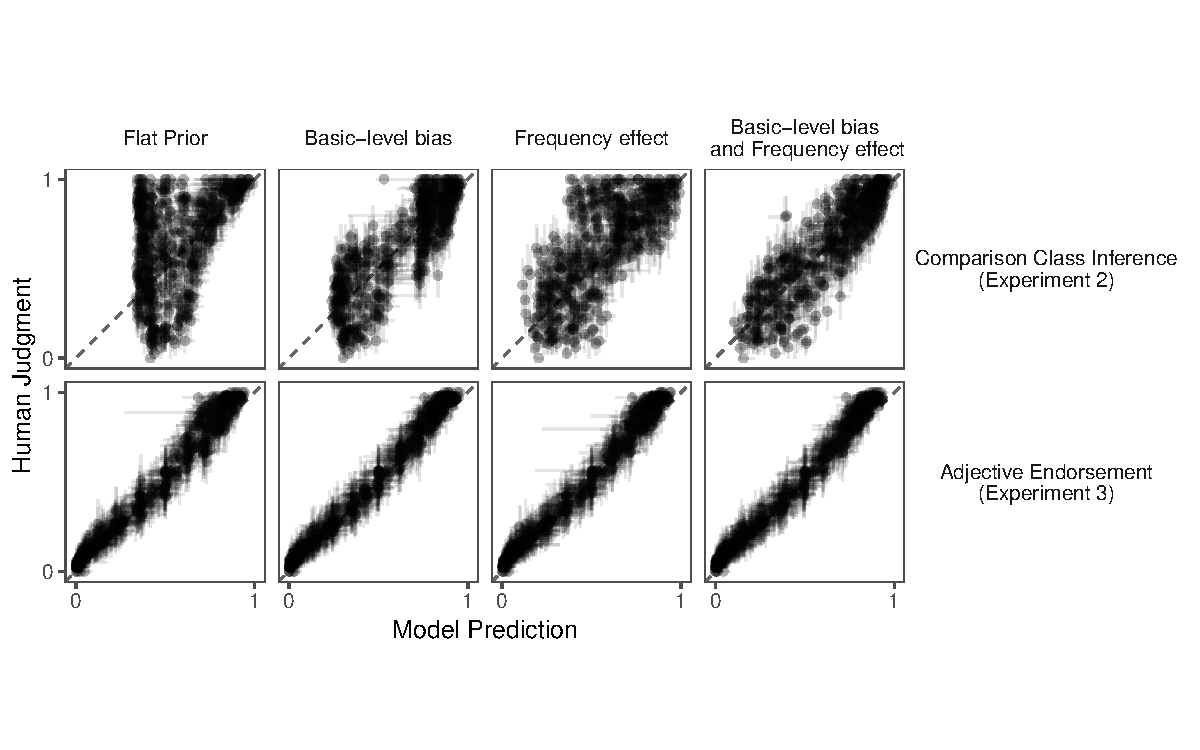
\includegraphics[width=\textwidth]{figs/model_scatters_modelVariants.pdf}
\caption{Model fits for Expt.~2 (Comparison Class Inference) and Expt.~3 (Adjective Endorsement) for four models that differ in their parameterization of the comparison class prior. Flat prior model assumes all comparison classes are equally likely a priori. Basic-level bias model assumes that there is a preference for a basic-level comparison class. Frequency effect assumes the prior probability of a comparison class tracks the frequency of the NP in a corpus. Basis-level and frequency effect assumes that the prior probability of a comparison class is a function of a basic-level bias and frequency. Dots represents means of the human judgments (proportion Specific-NP for Expt.~2; proportion endorsement for Expt.~3) and the maximum a-posteriori estimate of the model's predictions. Lines represents bootstrapped 95\% confidence intervals for the data and 95\% Bayesian credible intervals for the models.}
\label{fig:scatters}
\end{figure}
%We explore each of these components of the model to elucidate the cognitive representations that underly comparison class inferences.



%In addition to making qualitative predictions about the level-of-abstraction of the inferred comparison class, 
%\ndg{awk. the whole several layer intro to the bda is confusing and a bit redundant.}

All model variants are able to accommodate the norming, Adjective Endorsement data set well (Figure \ref{fig:scatters}, bottom row).
%The BDA models adjust the parameters of the world knowledge priors used in RSA in such a way as to make the adjectives felicitous for the categories in question; in this way, the adjective endorsement task (SI) serves as a norming data set. 
This result is a good sanity check; it shows that the adjective endorsement data is directly constraining the parameters of the world knowledge priors. 
We see this reflected in the imputed world knowledge priors, which reflect intuitively accurate general expectations about the categories (Figure \ref{fig:worldPriors}). 

The predictions of the different model variants come apart for the Comparison Class Inference data (Figure \ref{fig:scatters}; top row). 
The baseline Flat Prior model predicts variability in comparison class inferences only as a function of world knowledge about the properties, assuming all comparison classes are equally likely \emph{a priori}; this model explains roughly 17\% of the variance between items.
The Frequency effect model assumes NPs with higher usage frequency will more likely be used as comparison classes and is able to explain roughly 52\% of the variance.
The Basic-level bias model explains roughly 73\% of the variance by assuming that basic-level comparison classes may be more likely \emph{a priori}.
Finally, the maximally parameterized \emph{Basic-level and Frequency effect} -- a combination of the two alternative models -- gives rise to the best model predictions in terms of variance explained (78\%) and mean squared error (Table \ref{tab:r2bf}), suggesting that the structure of the comparison class reflects both a basic-level bias and an effect of the frequency of the NP, in addition to other possible factors. 

%Our BDA model returns posterior distributions over the parameters of the RSA models, governing world knowledge, the comparison class prior, and the speaker optimality parameters. 
%We first determine which parameterization of the comparison class prior (flat, basic-level bias, frequency, basic-level bias and frequency) is the best for our comparison class inference RSA model to predict the comparison class inference data. 
%We do so by examining the model's posterior predictive distribution over comparison class inference choices.
%The posterior predictive distribution marginalizes over the inferred values of the parameters to show what data the model would expect to see, given the parameters it has learned from the data. 
%Posterior predictive checks are an important step in model validation and provide a window into the model's strengths and shortcomings. 

%and (2) comparing the marginal likelihood of the data under each model to compute a Bayes Factor (BF) as a measure of formal model comparison. BFs quantify how well the model predicts the data, averaging over the prior distribution over parameters; by taking the average over the model's prior distribution over parameters, the measure explicitly takes into account model complexity because higher complexity models have wider prior distributions over the parameter \cite{lee2014bayesian}.


%\begin{figure}[t!]
%\centering
%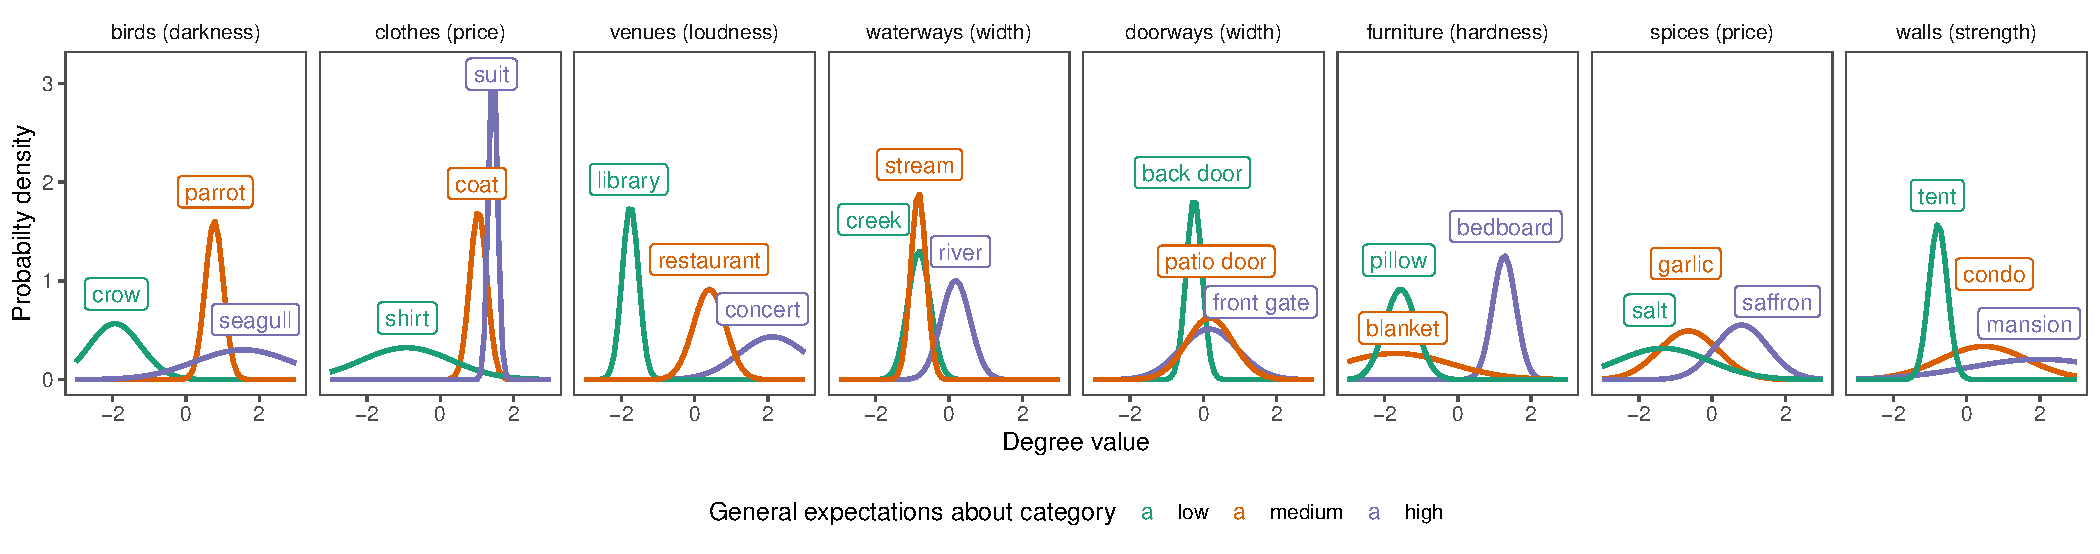
\includegraphics[width=\textwidth]{figs/reconstructed_world_priors.pdf}
%%{\centering 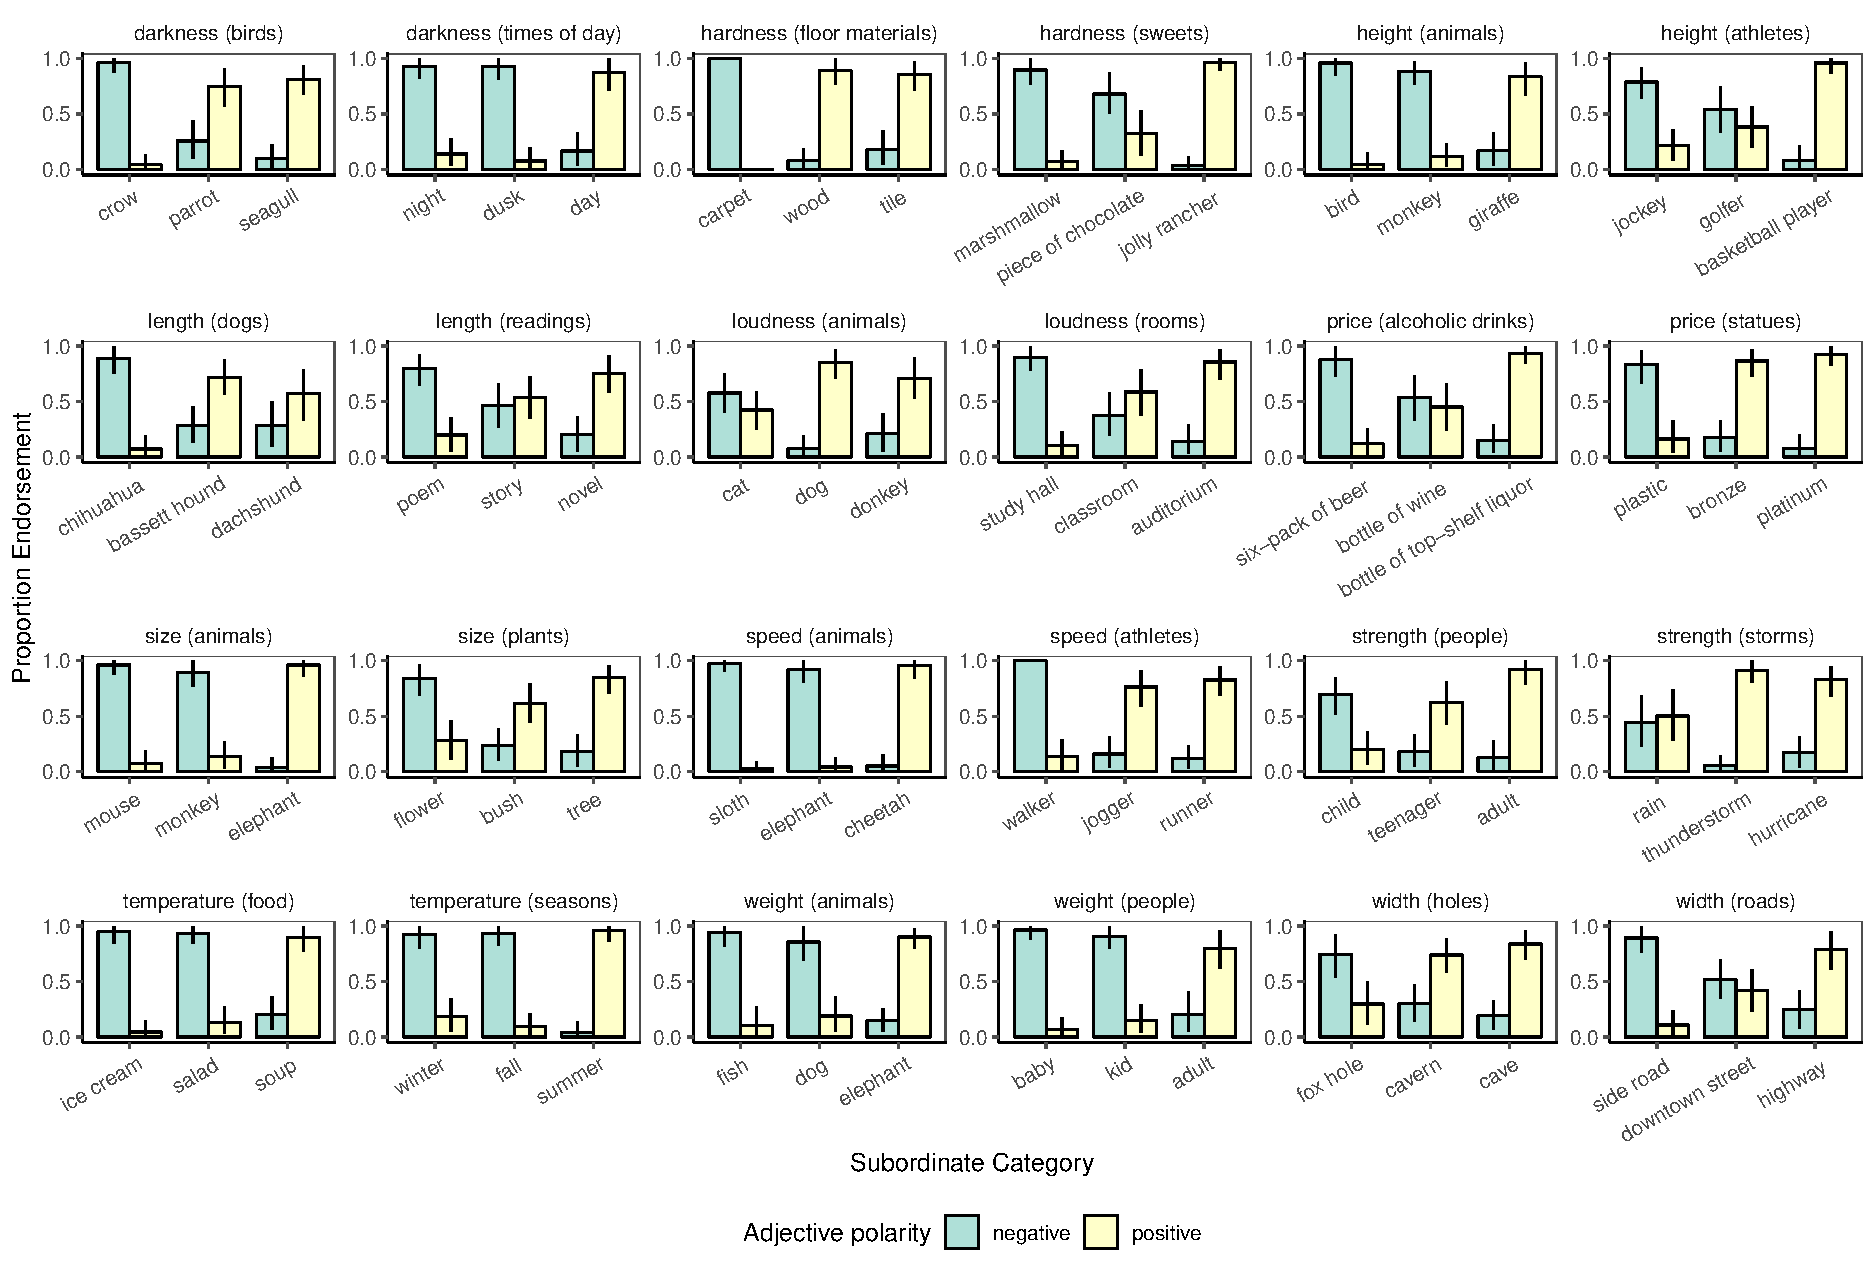
\includegraphics{figs/bars_adj_finalExpt_pilot_byItem} }
%\caption{xxx.}\label{fig:worldPriors}
%\end{figure}


\begin{figure}[t!]
    \centering
    \subfigure[Imputed prior distributions over degrees for 8 of the 90 item sets. These distributions were generated from the Maximum A-Posteriori parameter values inferred by conditioning on the Comparison Class Inference (Expt.~2) and Adjective Endorsement (Expt.~3)  data sets. See Figure \ref{fig:bayesnet} for full data-analytic model.]{\label{fig:worldPriors}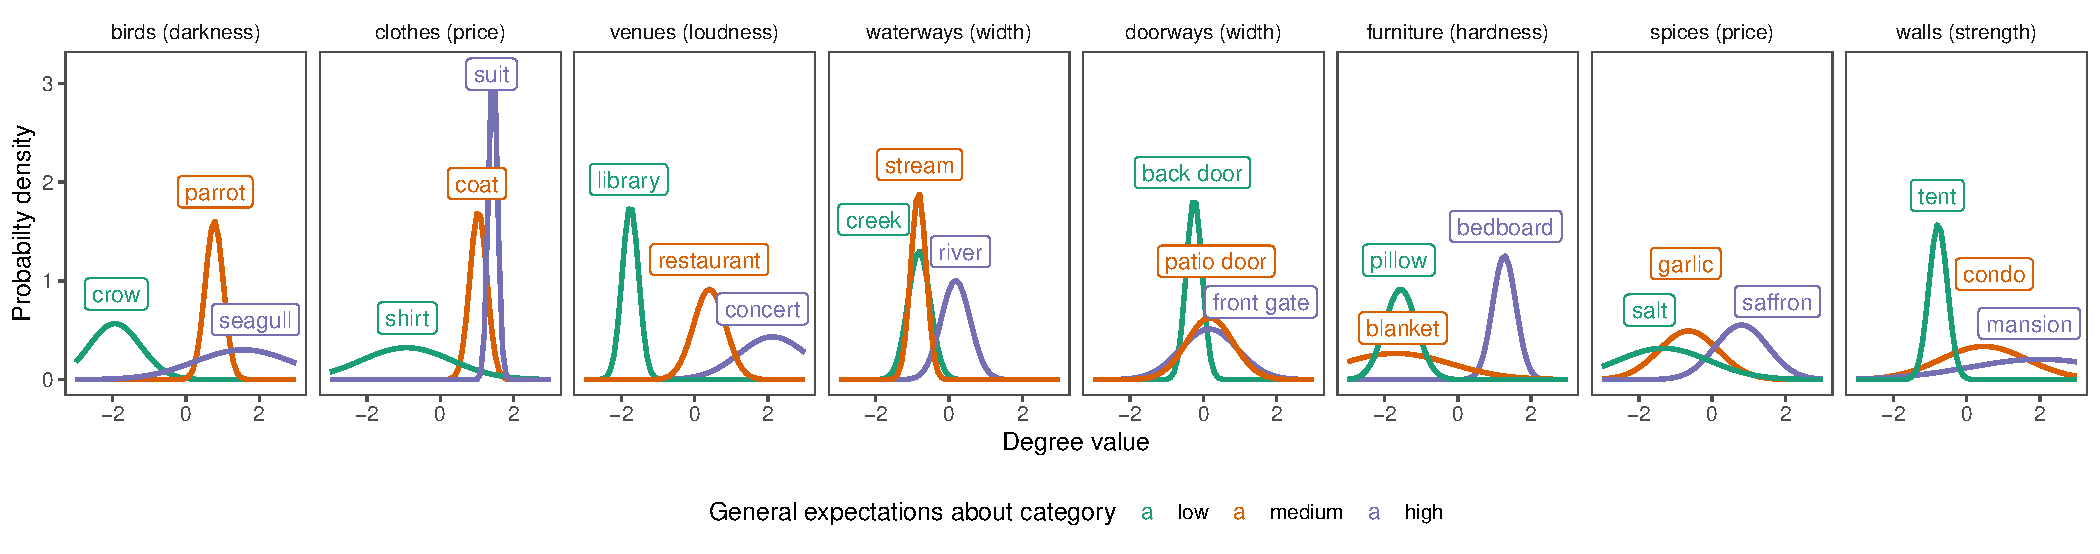
\includegraphics[width=\textwidth]{figs/reconstructed_world_priors.pdf}} \\
    \subfigure[Human data and model predictions for items with small residuals (left 4) and largest residuals (right 4). ]{\label{fig:residuals}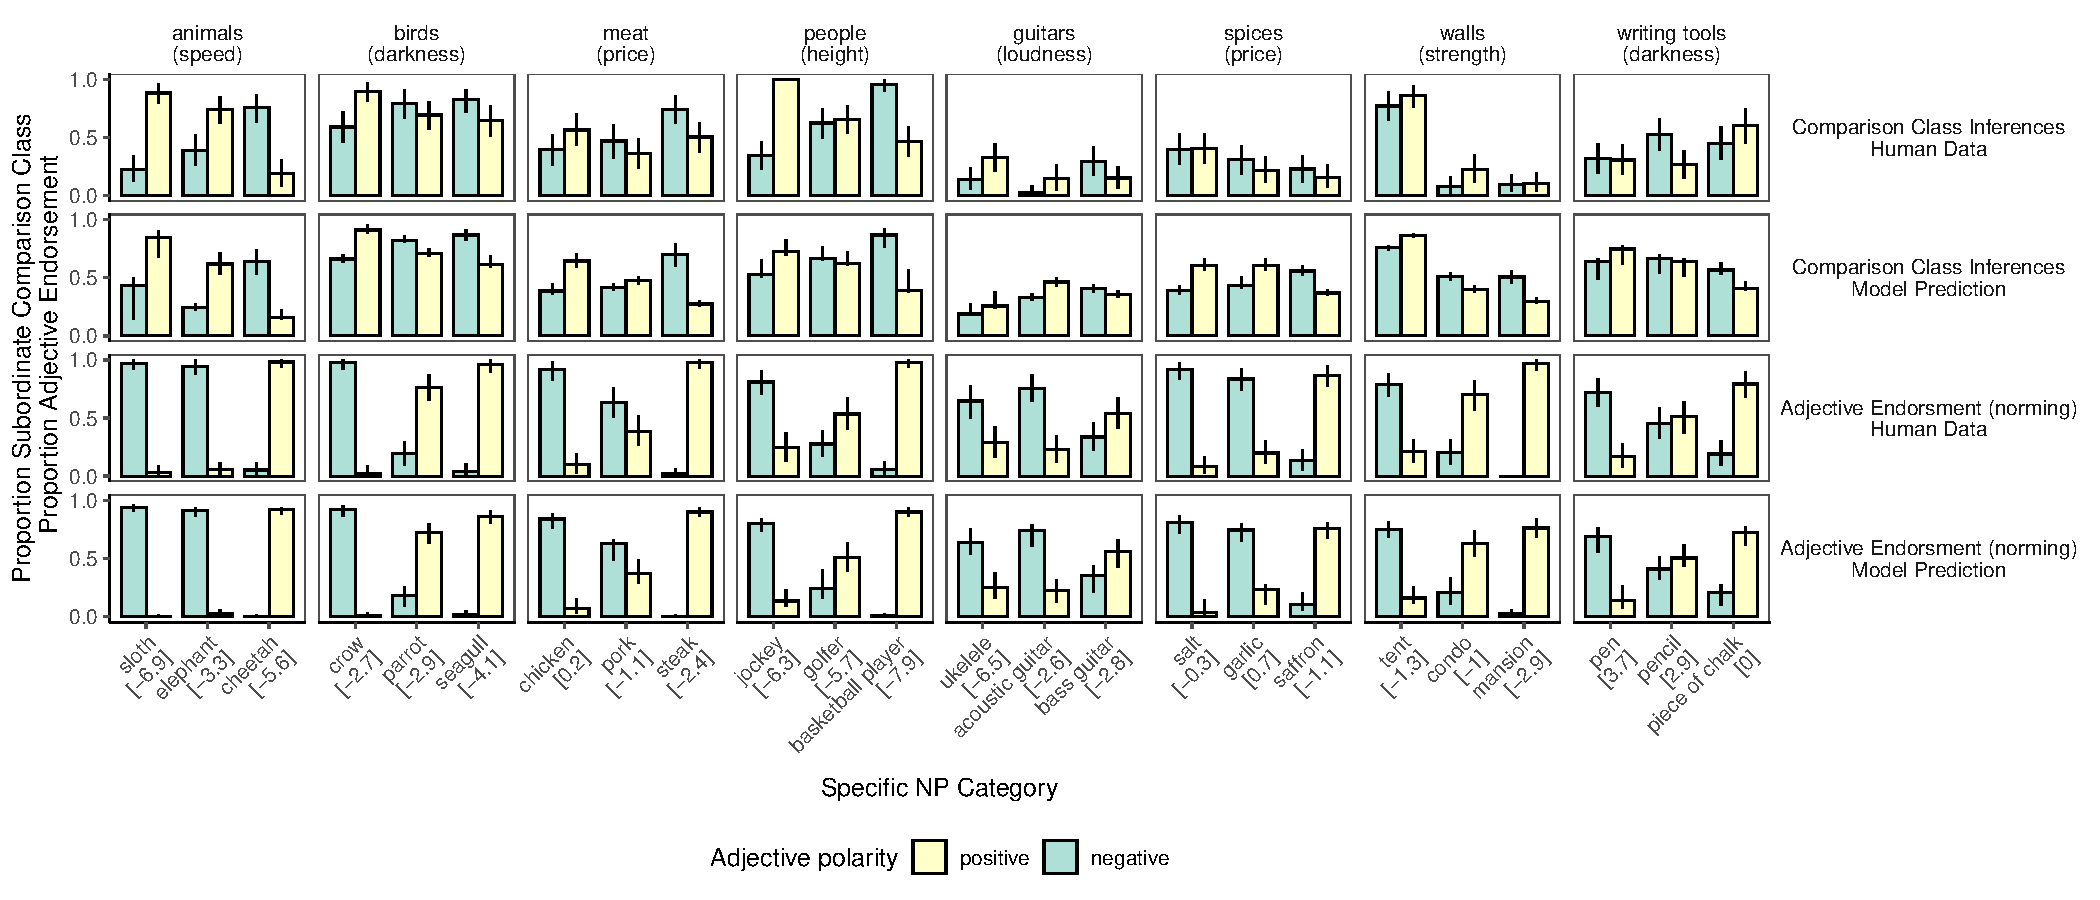
\includegraphics[width=\textwidth]{figs/bars_ccinfOnly_finalExpt_byNP_topResdiuals_intercept_slope_300k.pdf}}
    \caption{Quantitative modeling results.}
\end{figure}


%\begin{figure}[t!]
%\centering
%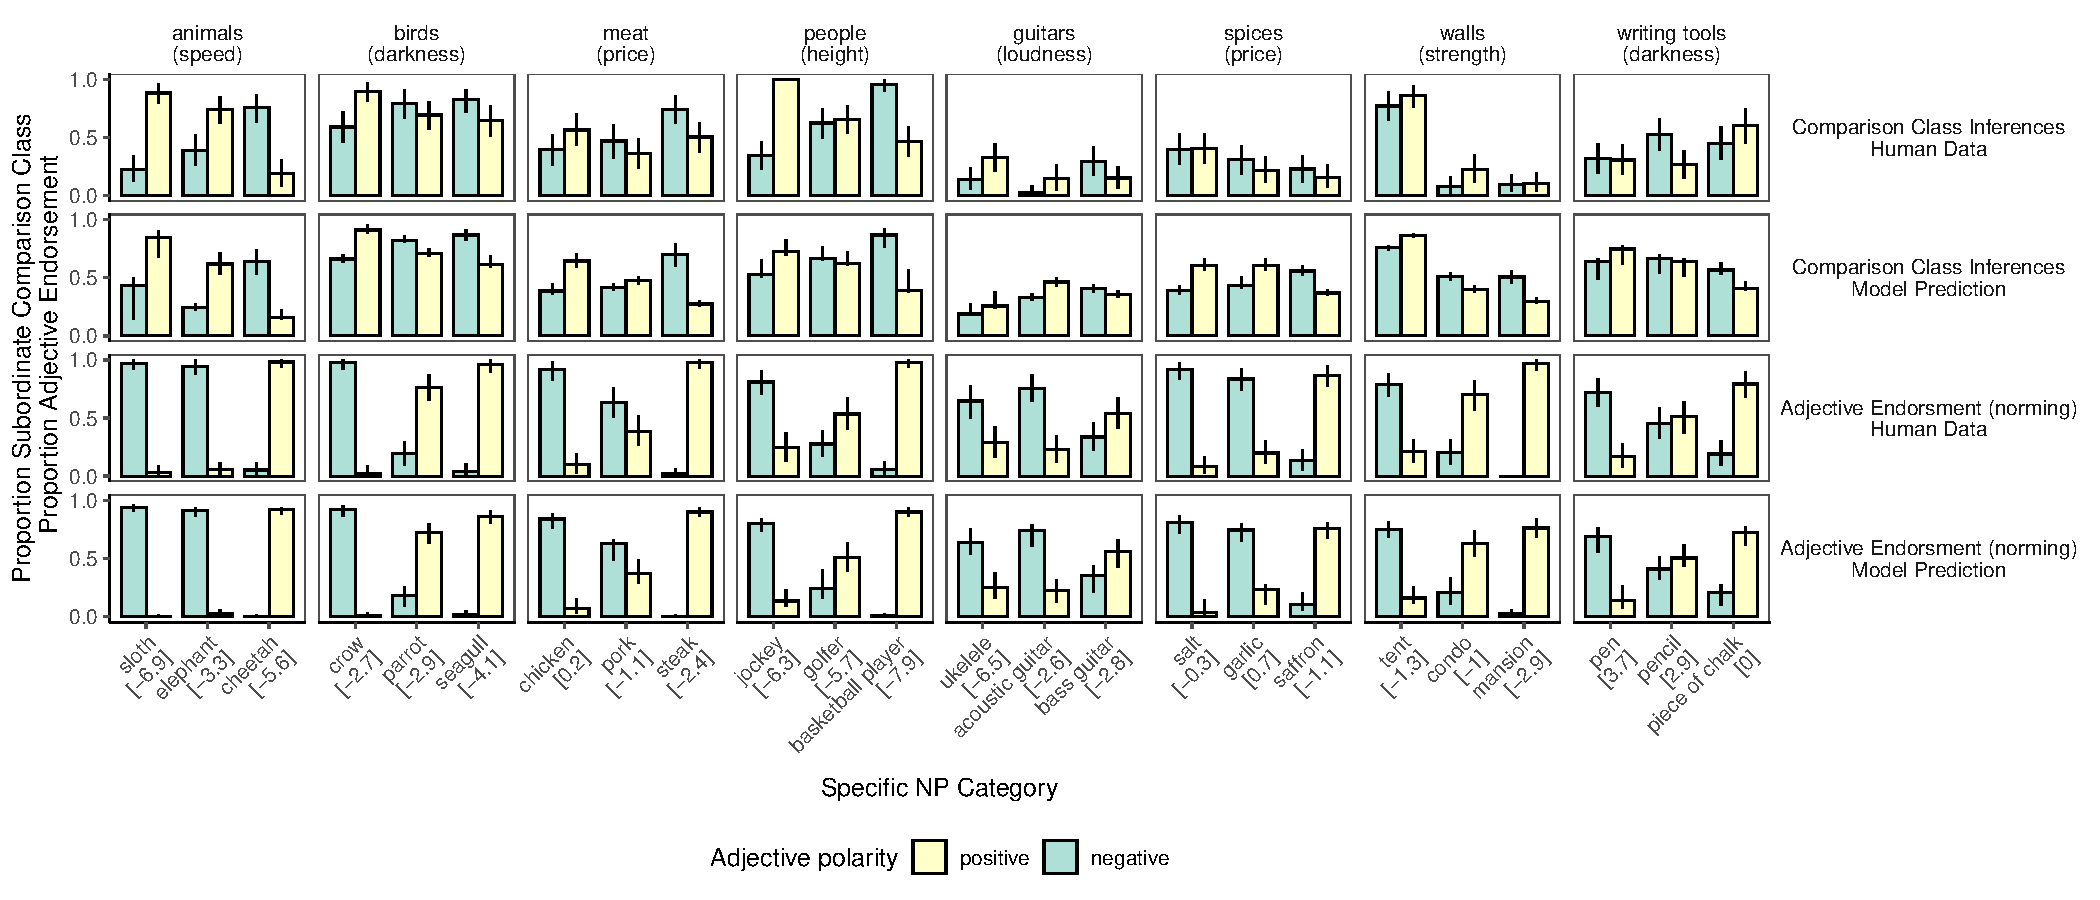
\includegraphics[width=\textwidth]{figs/bars_ccinfOnly_finalExpt_byNP_topResdiuals_intercept_slope_300k.pdf}
%%{\centering 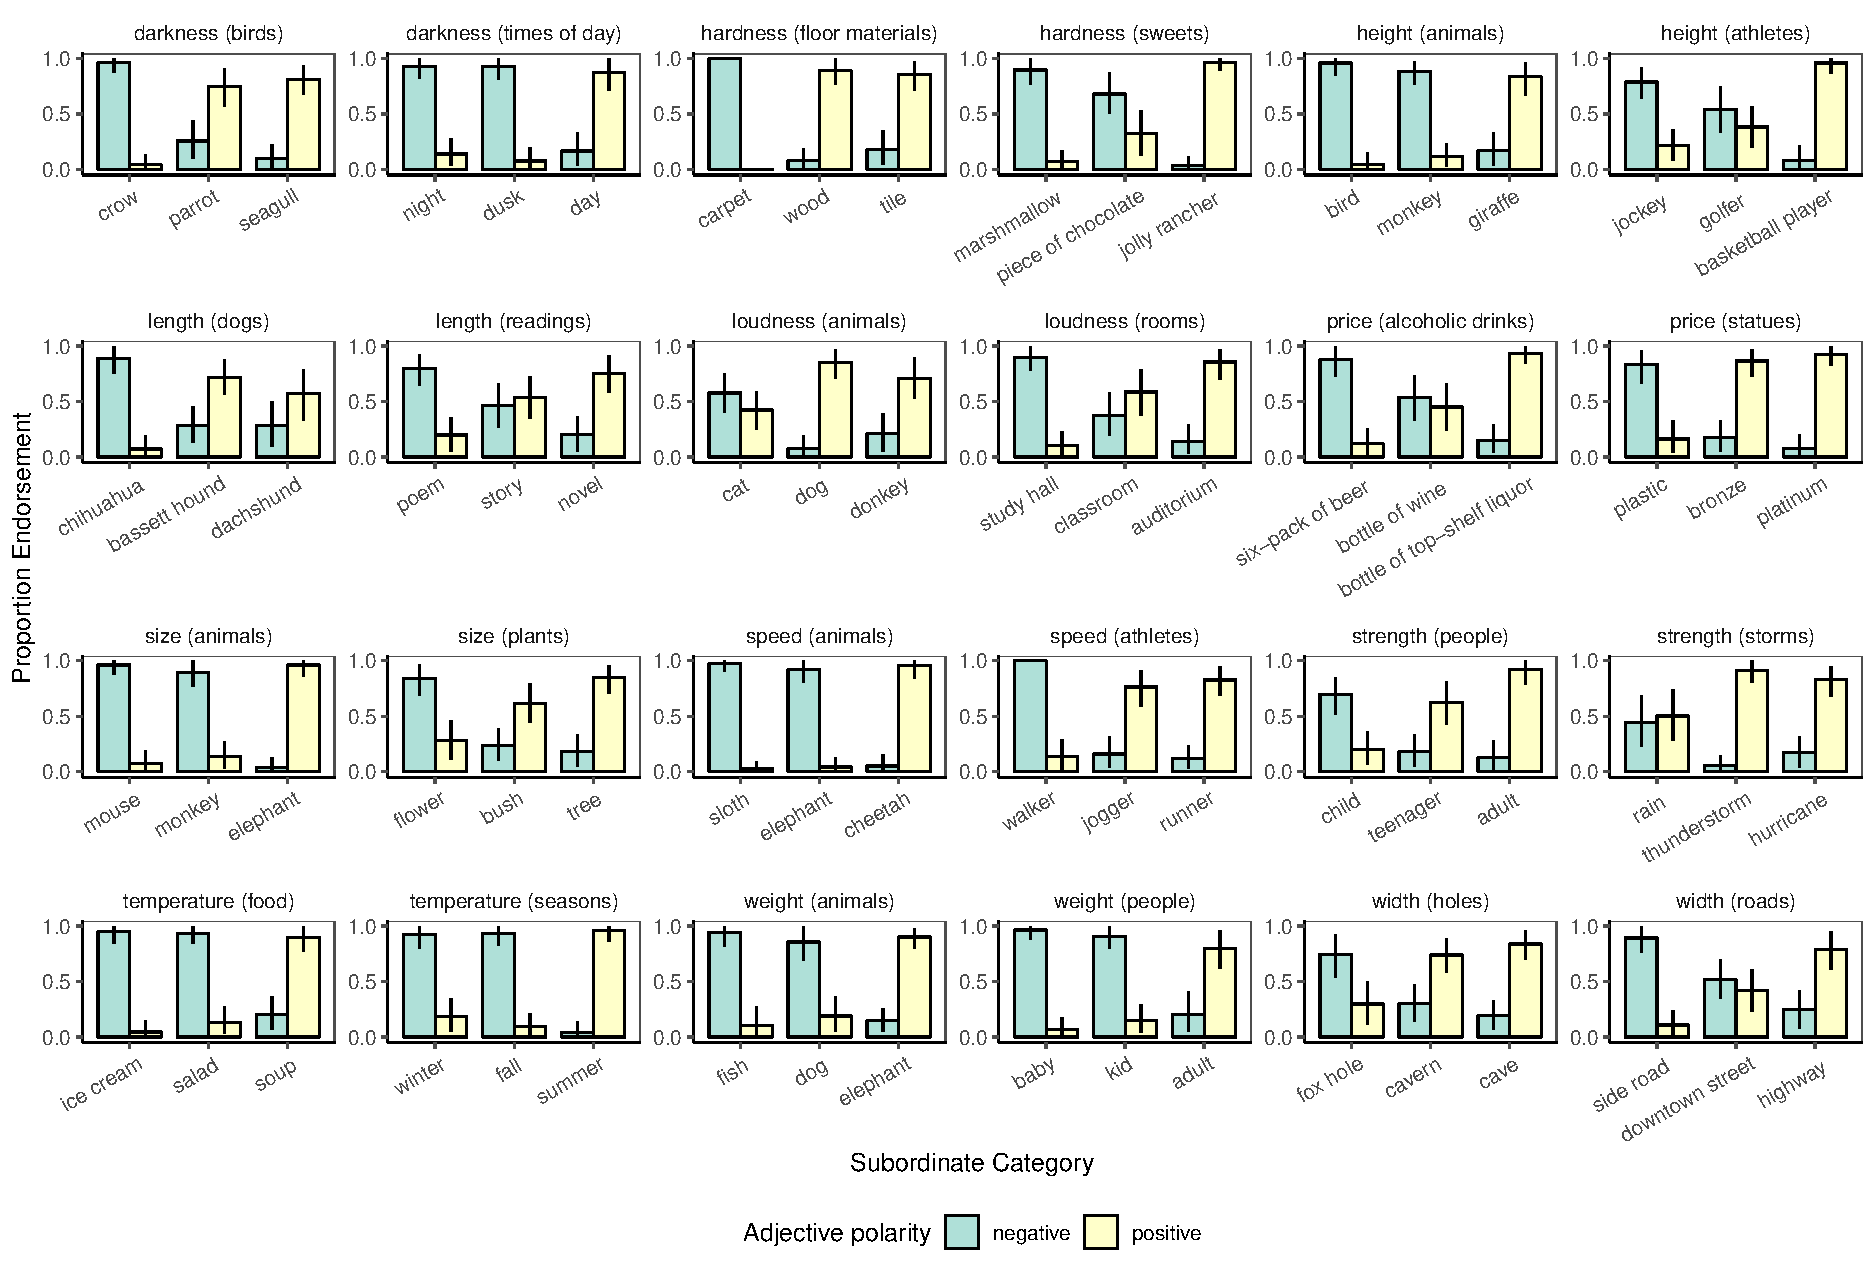
\includegraphics{figs/bars_adj_finalExpt_pilot_byItem} }
%\caption{Human data and model predictions for items with small residuals (left 4) and largest residuals (right 4).}\label{fig:residuals}
%\end{figure}


%The parameterization of the comparison class prior does not directly affect the model's predictions for the Adjective Endorsement (Expt.~3) data; these predictions are purely a function of the RSA model (see Supplement) and the distributional world knowledge used for both experiments (e.g., the distributions of heights for people). Thus, it is no surprise that all model variants do a good job at explaining the Adjective Endorsement data, and it is a good sanity check that the adjective endorsement RSA model is of the right form to accommodate the Adjective Endorsement data. 
%Our full model does a quite good job at accounting for the gradability of these inferences ($r = 0.88; r^2 = 0.77$)

To gain further insight into the comparison class inference results, we examine the maximal model's posterior distribution over parameters.
The speaker optimality parameters for each task were inferred to be values for which listeners assuming a rational speaker and consistent with the prior literature on RSA models --- means and 95\% Bayesian credible intervals: $\alpha_1 =  \hdiresults{model_params_cis.csv}{byItem-intercept_single-slope_speakerOptimality_subordinateCC_NA}$, $\alpha_2 =  \hdiresults{model_params_cis.csv}{byItem-intercept_single-slope_speakerOptimality_adjEndorse_NA}$.
We also find a positive effect of frequency of the noun phrase -- $\beta_1 = \hdiresults{model_params_cis.csv}{byItem-intercept_single-slope_beta_frequency_basic_super}$.
Our maximal model infers two parameters for the basic-level bias, one which operates if the particular item is a subordinate-level category (and thus, the more superordinate category would be the basic-level) and one that operates if the item is a basic-level category (and thus, the more superordinate category is the superordinate-level). 
We can then use those parameters to compute imputed prior probabilities of subordinate, basic, and superordinate comparison classes (assuming a constant effect of usage frequency). 
These parameters show that basic and subordinate comparison classes are highly accessible and superordinate comparison classes less so (Figure \ref{fig:parameters}).


%The full model infers on a by-item basis whether the basic-level category is the supplied NP or whether the basic-level category is an unmentioned, more superordinate category, because we expect the basic-level bias to operate differently for these different regimes of items.
%As expected, the comparison class prior NPs that were categorized as basic-level categories strongly favored those mentioned categories -- $\beta^1_0 = \hdiresults{model_params_cis.csv}{byItem-intercept_single-slope_beta_intercept_basic_super}$.
%For NPs that were categorized as subordinate categories (i.e., the basic-level category was an unmentioned, more superordinate category), the comparison class prior showed no appreciable basic-level bias -- $\beta^0_0 = \hdiresults{model_params_cis.csv}{byItem-intercept_single-slope_beta_intercept_sub_basic}$.
%From these parameters values, we can compute the overall imputed prior probabilities of subordinate, basic, and superordinate comparison classes (assuming a constant effect of usage frequency), which reflect the finding that basic and subordinate comparison classes are highly accessible and superordinate comparison classes less so (Figure \ref{fig:parameters}).
%and a positive effect of frequency of the noun phrase -- $\beta^0_1 = \hdiresults{model_params_cis.csv}{byItem-intercept_single-slope_beta_frequency_sub_basic}$.





\begin{center}
  \begin{table}[h]
    \centering
    \pgfplotstabletypeset[sci zerofill,
    col sep = comma,
    every head row/.style={before row = \toprule, after row = \midrule},
    every last row/.style={after row = \bottomrule},
    columns/model_variant/.style={string type, column name={Model}, column type = l},
    columns/subordinateCC_r2/.style={string type, column name={$r^2$ Expt.~2}, column type = l,  sci sep align, precision=3},
   columns/subordinateCC_mse/.style={fixed, column name={$MSE$ Expt.~2}, column type = l, dec sep align, precision=4},
    columns/adjEndorse_r2/.style={string type, column name={$r^2$ Expt.~3}, column type = l, sci sep align, precision=3},
     columns/adjEndorse_mse/.style={fixed, column name={$MSE$ Expt.~3}, column type = l, dec sep align, precision=4}]{csv_data_4_tex/mse_r2_table.csv}\caption{Model evaluation results. Full basic-level and frequency model exhibits the best fit to both data sets in terms of variance explained $(r^2)$ and mean squared error (MSE).}
    \label{tab:r2bf}
  \end{table}
\end{center}


\begin{figure}[t]
\centering
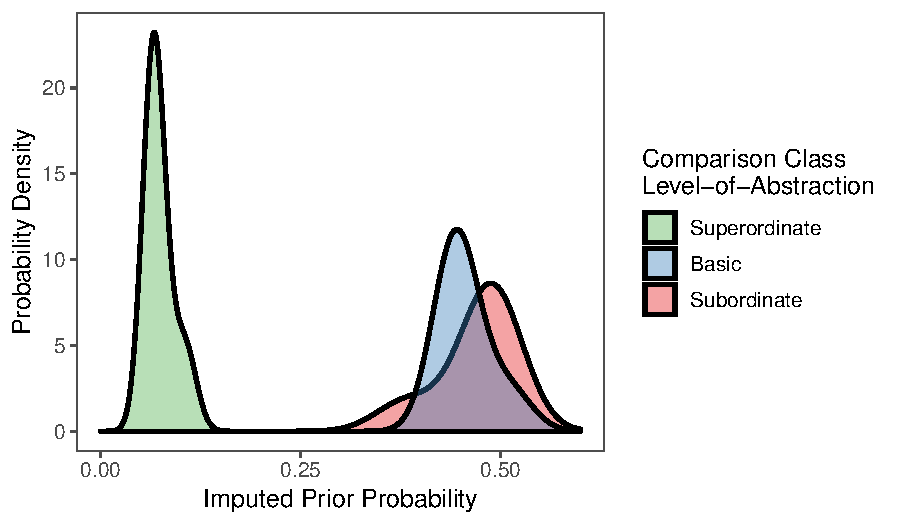
\includegraphics[width=0.7\textwidth]{figs/model_comparisonClassPriorParameters.pdf}
\caption{Imputed distributions over the prior probabilities of comparison classes at different levels of abstraction. Basic- and subordinate-level categories comprise \emph{a priori} likely comparison classes, while superordinate categories are less likely to serve as comparison classes.}\label{fig:parameters}
\end{figure}


 






%The full model's posterior over the RSA and data-analytic parameters were consistent with prior literature and intuition. The maximum a-posteriori (MAP) estimate and 95\% highest probability density (HPD) intervals for model parameters specific to the \(L_1\) model used for comparison class inference were \(\alpha^{1}_{1} = 1.60 [1.10, 2.50]\), \(\beta = 0.13 [0.11, 0.19]\). Model parameters specific to the \(S_2\) model used for adjective endorsement: \(\alpha^{2}_{1} = 3.50 [0.60, 13.20]\), \(\alpha^{2}_{2} = 3.20 [2.60, 3.80]\). The inferred distributions corresponding to subordinate class priors were consistent with the \emph{a priori} ordering of these subordinate classes (low, medium, high) used in these tasks (Figure \ref{fig:modelParameters} top).

%Finally, the full model's posterior predictive distribution does an excellent job at capturing the quantitative variability in comparison class inferences: \(r^2(30) = 0.96\), and adjective endorsements: \(r^2(30) = 0.98\) (Figure \ref{fig:posteriorPredictiveScatters}). Because of the overall preference for the subordinate comparison class, many of the data points are distributed above 0.5. Even for these fine-grained differences, the model does a good job at explaining the quantitative variability in participants' data (Figure \ref{fig:posteriorPredictiveScatters} right). Thus, the variability in comparison class inferences we observe in our behavioral data can be accounted for the constructs posited in our model (namely, the comparison class prior and degree priors).

\section{General Discussion}

%Inferring the comparison class from such a generative model goes beyond a model of concepts, however; listeners must reason about a speaker's behavior...


%
%
%This omission is problematic for 
%
%
%
%
%
%Theories of semantic composition for dealing with relative adjectives assume some comparison class.
%
%
%

%understand that \emph{big} is relative \cite{Sera1987} and that the
%comparison class can change





%Previous research has focused on what occurs during language understanding once a comparison class is determined.
%The question of how listeners decide upon a comparison class when it is not stated explicitly (e.g., ``It's warm relative to other days this winter'') has been addressed neither formally nor empirically.


%The speaker's choice of noun phrase can strongly influence the comparison class  (e.g.,  a \emph{big snowman} is probably big relative to other snowmen), though it need not determine it: saying ``That's a big snowman'' to a 4-year-old might mean \emph{big relative to snowmen a 4-year-old could build} \cite{kamp1975two}. 
 
% In this paper, we investigate the first aspect of this open-ended inference problem, deciding among multiple possible comparison classes. 


%The existence of comparison classes for understanding relative adjectives is uncontroversial \cite{cresswell1976semantics, klein1980semantics, kennedy2005scale, bale2008universal, Bale2011, Solt2009}. %\red{more standard citations for this?}



Interpreting language requires understanding the context in which the words are uttered.
Yet, speakers almost never articulate context explicitly but leave it to the listener to pragmatically reconstruct. 
Inferring comparison classes for relative adjectives (e.g., \emph{tall}) is a case study in this larger phenomenon of the pragmatic reconstruction of context.
In this paper, we find that listeners flexibly adjust the comparison class using pragmatic reasoning and world knowledge, which we predict with a state-of-the-art model of language understanding and empirically confirm with an open-ended response measure on a diverse range of stimuli.

We propose a minimal extension to an adjective interpretation Rational Speech Act model to allow it to flexibly reason about the implicit comparison class (e.g., \emph{tall for a person}~vs.~\emph{tall for a basketball player}).
The model generated the qualitative prediction that listeners should prefer more specific (e.g., subordinate-level) comparison classes when the adjective conflicts with their general expectations about a member of a category (e.g., a basketball player who is short), which we confirmed using a free-production measure.
The fact that participants naturally produce different responses to the our comparison class elicitation task suggests that these inferences are easily accessible and can arise spontaneously.
%and we showed how this inference requires pragmatic reasoning; a literal interpretation model in fact draws the wrong inference.
The model also made quantitative predictions about the gradability of this inference given knowledge about properties and categories. 
The strong quantitative fit of this model to the free-production data provides compelling evidence that the comparison class inference can be viewed as a pragmatic inference formalized using the machinery of probabilistic reasoning.

Though our fully parameterized model does the best job at accounting for the variability in comparison class inferences, the data set exhibits even more variability than our model can account for. Figure \ref{fig:residuals} shows the four item sets with largest mean model residuals (as well as the four item sets with smallest mean model residuals).
The model struggles to match participants' inferences for \emph{spices}, which do not show the predicted effect of expectations and also show a fairly strong basic-level bias for the more superordinate category of \emph{spices}. 
In our maximal model, we an overall weak preference for basic-level categories over subordinate level categories and so the model does not show a strong preference for \emph{spices}. 
A similar pattern can be observed for the doorways item and the condo and mansion wall items, where human inferences much more strongly support the more superordinate categories than the model's inferences. 
These cases are all artifacts, suggesting that the effect of the basic-level on comparison class inferences may be different for artifacts as for animals, perhaps owing to differences in conceptual representations of these higher-order categories \cite{gelman1988development, kalish1998natural, rhodes2009developmental}.
%Spices: garlic is more like salt, but people have a strong preference for "spices" here... because sub and basic level categories are assumed to have equal probability, we fail here. 


Previous work investigating the role of the comparison class in adjective interpretation has provided strong linguistic cues to convey the speaker's intended comparison class. 
\citeA{Barner2008} were able to convey to 4-year-olds that the comparison class for a ``tall pimwit'' is \emph{other pimwits} and does not include other non-pimwit objects.
\citeA{Ebeling1994} showed how even younger children can flexibly shift between qualitatively different kinds of comparison classes, given strong linguistic cues to distinguish the intended comparison class (e.g., ``Is this a \emph{big mitten}?'' vs. ``Is this mitten \emph{big for a doll}?'').
In our experiments, the speaker does not use a category label (e.g., ``basketball player'', ``winter'') in their utterance (e.g., ``He's tall''; ``It's warm''); without these strong linguistic cues, adults flexibly adjust the comparison class by using their world knowledge. 
The fact that young children, who do not have the same kind of world knowledge as adults, can flexibly adjust the comparison class raises the question of what kinds of cues are available to them (and to adults) in the naturalistic environment to use to infer the comparison class.

%\mht{minimal cues... also, NP $\neq$ cc}
%A relevant detail of our experiment contexts is that the speaker's sentence did not include a noun phrase to describe the referent (i.e, the speaker said ``He is tall'' as opposed to ``That basketball player is tall''). 
%We found that when the adjective is consistent with the listener's general expectations about the category (e.g., the basketball player is tall), listeners prefer comparison classes that are also more general (i.e., tall for a person). 
%Intuitively, the speaker's intentional production of a noun phrase could more directly communicate the comparison class by revealing how the speaker is conceptualizing the referent (e.g., \emph{the speaker is conceiving of this person as a basketball player}).
%The extent to which this inference holds could also depend upon the syntactic structure of the sentences: 
%Prenominal uses of the adjective (e.g., ``He's a tall basketball player'') might be an even stronger cue. 
%Indeed, prenominal uses are argued to be ideal for a child learning the meaning of novel adjectives \cite{Waxman2001, Mintz2002, Sandhofer2007} perhaps because it is such a strong cue to the comparison class.
%Future work should investigate the interaction between syntactic structure and pragmatic inferences regarding the comparison class.

The phenomenon of comparison class inference is a case study in \emph{context inference}, or reasoning about the set of beliefs that are in common ground between speaker and listener.
%Our model is similar in structure to 
The model may thus be similar in structure to models of presupposition accommodation, which linguistic theories classically pose as involving a listener adding or revising information to the common ground in order to make sense of an utterance. For example, if John says to Mary ``My car is in the shop'', it is not necessary \emph{a priori} that Mary know that John has a car; if Mary did not know (or she temporarily forgot) that John owns a car, Mary can \emph{accommodate} John's utterance by adding to the common ground the presupposition that \emph{John has a car}. 
In our case, the speaker utters an adjectival sentence without a strong cue to the comparison class: \emph{He [a basketball player] is tall}. 
A speaker would only utter such a sentence if they believed either (i) the comparison class was already in the common ground or (ii) the listener can reasonably be assumed to infer the comparison class.
The utterance makes sense either if the comparison class is \emph{people} or \emph{basketball players}, but it is comparatively more likely to be true if the comparison class is \emph{people}. 
In the Computational Model section, we showed how the inference about the comparison class goes through regardless of whether the listener assumes the speaker was presupposing the comparison class to already be in the common ground or if they assumed the listener could reconstruct the intended comparison class.
The continuity in the computational mechanisms that underly this sort of common ground revision 
 
%The situation we model is one of asymmetric knowledge: The listener is uncertain about the comparison class, but assumes that the speaker does not represent their uncertainty. 
%The comparison class assumed by the speaker, then, acts as a kind of presupposition, and for the formal modeling mechanism we employ has in fact been deployed in modeling presuppositions \cite<e.g., ``When did John quit smoking?'' implies that John used to smoke;>{Qing2016projective}.
%In our experiment, the speaker is talking to a third party and the actual comparison class inference may be a result of the participants' uncertainty about the information in common ground between the interlocutors; future work should examine dyadic interactions to better understand the role of asymmetric knowledge in inferring comparison class.
%\mht{relation to accommodation... pretend as if i the listener didn't know the referent was a basketball player}
%comparison class most likely to make the utterance true while
%prioritizing more specific (lower variance) classes because they are
%more informative. It also made quantitative predictions about how
%background knowledge about the degree scale and what classes are likely
%to be talked about \emph{a priori} should inform this inference in a
%graded fashion. Both qualitative predictions of the model were borne out
%in our behavioral experiment, and the quantitative predictions were
%confirmed using a novel data analytic technique.


Comparison classes are useful because they allow us to generalize the lexical semantics of many different kinds of adjectives and other linguistic messages that convey \emph{relative} meanings. 
For example, the meaning of \emph{tall} and \emph{warm} have equivalent functional forms, which vary only in the dimension the adjective picks up: $\denote{tall} = \text{height}(x) > \theta$ and $\denote{warm} = \text{temperature}(x) > \theta$. 
Human cognition can use the minimal semantic template---$\denote{adj} = \text{dimension}(x) > \theta$---and infer the intended comparison class (which determines $\theta$) to create an infinity of possible meanings.
Such simple semantic representations, coupled with a powerful inferential cognitive mechanism, could help explain why young children acquire such context-sensitive language (e.g., the word \emph{big}) so early \red{(cite acquisition lit)}: General purpose inferential mechanisms can be used to determine the comparison class, thus filling in a large part of the meaning in context. 

%This problem of inferring comparison classes is closely tied to the problem of inferring the intended referent, or deconstructing how the speaker is conceptualizing the referent, of an utterance.
%For example, ``That's a beautiful cat'' could be said felicitously of a drawing of a cat, in which case, the comparison class is \emph{drawings of cats}; thus, the meaning of ``cat'' in the original utterance should be understood as \emph{drawing of a cat} and not an actual cat.
%In a similar way, inferring that the speaker meant the basketball player is short \emph{for a basketball player} might be tantamount to inferring that the speaker is conceiving of the referent as a basketball player. 
%This potential symmetry between comparison classes and representations of referents could have implications for theories of alternative utterances: For example, the speaker said ``cat'' and not ``drawing of a cat'' because they believed the listener would not be confused, given the context, that the referent is not an actual cat. 

We have addressed a particular aspect of comparison class inference: deciding among multiple possible conceptually-based comparison classes. 
Other kinds of comparison classes are possible (e.g., perceptually-based comparisons and functional comparisons as in ``big for the doll'') and are understood by even very young children \cite{Ebeling1994}.
The inferential machinery we present in our model of comparison class inference is general and should apply equally well to these other kinds of comparison classes, once a hypothesis space of comparison class is determined.
Determining this hypothesis space of comparison classes is an important future direction for this approach. 
For example, how do we know to even consider the comparison classes of basketball players vs. people, and not all objects in general? 
\emph{Objects} may be a comparison class that listeners would consider given the right context and our assumption of constructing comparison classes out of a taxonomic hierarchy is consistent with \emph{objects} being a candidate comparison class.
However, just because a comparison class is in the hypothesis space does not entail that is a likely comparison class: Indeed, we observe in our quantitative modeling results that a uniform prior distribution over comparison classes is unlikely, and in fact, superordinate categories have the lowest probability of providing the comparison class. 
The fact that superordinate categories are dispreferred may be a product of the fact that superordinate categories tend to have higher variability across members than basic-level or subordinate level categories. 
Our modeling work also shows that usage frequency of the noun phrase contributes to the comparison class prior. 
Corpus frequency is a composite measurement of factors relevant for speech production. 
Its utility in this model suggests that utterances without an explicit comparison class (e.g., ``It's warm outside'') may in fact be elliptical sentences, in a way analogous to sentence fragments studied in noisy-channel models of production and comprehension \cite{bergen2015strategic}. 

%Our solution at present is to say that \emph{objects} is a comparison class with low probability, but why should it have low prior probability?
%From our modeling work, we found that the \emph{superordinate} level was the least likely to give rise to a comparison class, and that may result from superordinate categories having a 
%\mht{Show simulations of comparison class inference with classes that have same mean but increase in variance?}
%For example, the comparison class of ``people'' for heights of individuals is relatively more salient than the class of ``produce'' (or, ``fruits and vegetables'') for the weights of particular fruits and vegetables. 
%As a proxy for the prior probability of a comparison class, we used a (logistic) linear function with an intercept to reflect a basic-level bias \cite{rosch1975family} and a slope of the frequency of the noun phrase in a corpus. 



%\mht{relation to  the inference about the comparison class being ``the speaker is thinking of the referent as an X''... reduces to same thing?}

In addition to the novel empirical data and the computational model of comparison class inference, this paper also presents experimental and data-analytic methodological innovations. 
On the experimental side, we articulated an explicit generative model of our items, which we deployed on human participants to construct a large and diverse set of linguistic stimuli (n = 540 unique stimuli). 
While this procedure was not entirely ``end-to-end'' (i.e., we authors still needed to curate, edit, and add context to the items), the method presents a significant advance beyond the traditional method of constructing a small set of stimuli, often inadvertently optimized to test a theory \cite{Clark1973}.
On the data-analytic side, we coupled a \emph{descriptive Bayesian} approach \cite{tauber2017} with the productivity of probabilistic models of language understanding \cite{Goodman2016, scontras2017probabilistic} to jointly model two complementary language tasks and infer the relevant prior knowledge shared between the tasks.
The major feature of this method is that it allows us to back-out quantitatively detailed domain knowledge that would be otherwise inaccessible through traditional prior elicitation techniques because human participants lack requisite knowledge of the quantitative scales (e.g., how many decibels is the sound of a rooster's crow?); in addition, this method has the feature that  participants respond only to simple, natural language questions rather than estimate numerical quantities for which complicated linking functions must be designed \cite<cf.,>{Franke2016}. 
The fully Bayesian language approach we pioneer here also provides further constraints on the language understanding models, which must predict quantitative data from two similar but distinct language experiments. 
The productivity of natural language can thus be harnessed to productively design experiments that further constrain and test computational models of language and cognition.


%It's been suggested that there exist qualitatively different kinds of
%comparison classes, constructed by reference to either: the perceptual
%context (a \emph{perceptual comparison class}), a goal of an agent or
%intended use of an object (a \emph{functional comparison class}), and
%the kind of the referent (a \emph{conceptual comparison class}; Ebeling
%\& Gelman, 1994). In this paper, we investigated the latter, but the
%question remains about how a listener should decide to switch between
%different kinds of comparison classes. For example, if Ann and Carl are
%deciding what to do on a Friday night, Carl suggest the ballet, to which Ann replies ``The
%ballet is expensive'', Carl should understand Ann's statement relative
% \emph{other ways they could spend their Friday night}, a kind-of
%functional comparison class. Goal inference is thus an associated
%ingredient in comparison class inference, and integrating the two
%should be a target for future work.





%Investigations of how human listeners understand vague adjectives have
%shed light on the precise mechanisms by which people interpret
%context-sensitive language, but have had little to say about how
%listeners decide upon what counts as the appropriate context. In this
%paper, we take the first step towards investigating the flexibility in
%the class against which an entity can be implicitly compared, a very
%basic form of context. Resolving underspecification by means of a comparison is not unique to
%\emph{gradable adjectives} like ``big'' or ``tall'', but is
%a general problem for language understanding. ``John ate \emph{a
%lot} of hot dogs'' probably means four or five hot dogs, whereas
%``John ate \emph{a lot} of potato chips'' could imply a quantity
%over a hundred (Schöller \& Franke, 2017); ``Robins lay eggs''
%means roughly that \emph{female robins} lay eggs, whereas
%``Robins fly'' entails something stronger, most or all robins fly
%({\textbf{???}}; {\textbf{???}}). Even noun concepts (e.g.,
%``furniture'') are graded (Rosch \& Mervis, 1975) and can be made
%more precise in context. Investigating how listeners interpret words
%like ``big'' is thus a case study of a crucial, general problem in
%language understanding: Understanding context-sensitive language.
%
%We investigated the question of how a listener decides among multiple
%possible conceptually-based comparison classes (e.g., tall for a
%basketball player vs.~tall for a person). It is notable that our model
%was able to account for inferences about items that did not fall into
%strict hierachies (e.g., \emph{movies} is not subordinate to
%\emph{things you watch online}) as well as items that did (e.g.,
%basketball players and people). This result suggests that our modeling
%framework can easily extend into cross-cutting comparison classes (e.g.,
%\emph{men}, \emph{people of a certain age}, \emph{basketball players}).
%
%\subsection{The phenomenon of comparison class
%inference}

%\subsection{Comparison class prior}
%
%We observe in our quantitative modeling results that a uniform prior
%distribution over the experimentally supplied comparison class
%alternatives is unlikely (Figure \ref{fig:modelParameters} bottom). For
%example, the comparison class of ``people'' for heights of
%individuals is relatively more salient than the class of
%``produce'' (or, ``fruits and vegetables'') for the weights
%of particular fruits and vegetables. We used the frequency of the class
%in a corpus as a proxy for their prior probability \(P(c)\), which was
%sufficient to account for differences in baseline class probability both
%\emph{between}- and \emph{within}-scales.
%
%Corpus frequency is a composite measurement of factors relevant for
%speech production. Its utility in this model suggests that utterances
%without an explicit comparison class (e.g., ``It's warm outside'')
%may in fact be incomplete sentences, in a way analogous to sentence
%fragments studied in noisy-channel models of production and
%comprehension (Bergen \& Goodman, 2015). Another (non-mutually
%exclusive) possibility is that the comparison class prior reflects
%basic-level effects in categorization (Rosch \& Mervis, 1975). Future
%work should attempt to understand these factors to construct a more
%complete theory of the comparison class prior.
%


\section{Conclusion}

The words we say are often too vague to have a single, precise meaning,
and only make sense in context. The context, however, can also be
underspecified, leaving the listener in the dark about both the
speaker's intended meaning and about the context through which the
listener is to make sense of the conversation. This work suggests that listeners infer a lot from a little:
The meaning and the context from a single vague utterance.


\section{Acknowledgements}

This work was supported in part by NSF Graduate Research Fellowship
DGE-114747 to MHT and a
Sloan Research Fellowship, ONR grant N00014-13-1-0788, and DARPA grant
FA8750-14-2-0009 to NDG.

\newpage


\bibliographystyle{apacite}

%\setlength{\bibleftmargin}{.125in}
%\setlength{\bibindent}{-\bibleftmargin}

\bibliography{comparison-class}

\newpage

\section{Supplementary Methods}

\subsection{Task 1: Stimuli Generation}

\subsubsection{Participants}

We recruited 50 participants from Amazon's Mechanical
Turk, restricted to those with U.S. IP addresses with at least a
95\% work approval rating. The experiment took about 5 minutes and
participants were compensated \$0.60 for their work.

\subsubsection{Materials}

We used 15 pairs of positive- and negative-form gradable adjectives that describe physical dimensions (Table \ref{tab:1}).
Some of the adjective pairs described the same dimension and/or had an adjective in common with another pair (e.g., \emph{fast}--\emph{slow} and \emph{quick}--\emph{slow}); these were included because we believed they would bring to mind different kinds of categories.

\subsubsection{Procedure}

On each trial, participants were given a phrasal template, for which they were asked to fill-in the missing elements.
The template was composed of three sentences, each missing a subject; the content of the sentence described the subject as one generally having the adjective applied to them (Figure \ref{fig:exptOverview}, Step 1). 
These sentences were followed with another that said that the three kinds of subjects from the previous sentences were all instances of a more general category: ``all kinds of \_\_\_''.
This last sentence was introduced to constrain the kinds of responses to the first three sentences such that the subjects would be all members of the same basic- or superordinate level category. 

The template for ``big'' and ``small'' looked like: 
\begin{description}[noitemsep]
%\tightlist
\item \_\_\_\_\_ are generally big.
\item  \_\_\_\_\_ are generally small.
\item \_\_\_\_\_ are sometimes big and sometimes small.
\item These three are all kinds of \_\_\_\_\_.
\end{description}
%
Participants filled out one template for each of the 15 pairs of adjectives. 


\subsubsection{Results}
From the full set of responses (750, in total), we select sets of items to be used in the subsequent experiments. 
We selected item sets on the basis of hierarchal consistency of the categories (i.e., that the three generated categories corresponded to the same level of abstraction e.g., they were all subordinate categories of the same basic-level category) and based on how well the items would make sense in the kinds of minimal contexts we use in Expt.~2. 
Two examples from each adjective pair are shown in Table \ref{tab:1}. 
We code each of the subordinate categories as to whether they were expected to fall low, high, or in the middle of the degree scale (i.e., those generated in response to the \emph{generally positive adjective}, \emph{generally negative adjective}, or \emph{sometimes positive and sometimes negative}). 


\subsection{Task 3: Adjective endorsement details} 

This experiment served to generate further data that could be used to constrain the model parameters shown in Figure \ref{fig:bayesnet}.
Sample size, sampling procedure, exclusion criteria, and data analysis were preregistered: \url{osf.io/vdkbp}.

\subsubsection{Participants}

We recruited 300 participants from Amazon's Mechanical Turk, restricted to those with U.S. IP addresses with at least a 95\% work approval rating. 
This number was arrived at with the goal of estimating endorsement probabilities for each item with a 95\% confidence interval width of 0.2 for each item. 
Because our measure is a two-alternative forced-choice and because we expect some items to receive fairly categorical judgments (i.e., low between-participant variability), we employed a sequential sampling procedure in order to over-sample items that exhibit non-categorical judgments (i.e., high between-participant variability). 
We first collected 35 responses for each item, computed 95\% CIs for each item, and stopped collecting data for items whose 95\% CIs were smaller than 0.2.
After the first 35 responses, we collected more responses for each item until the 95\% for that item was smaller than 0.2 or we reached our predetermined sample size. 
The experiment took about 10 minutes and participants were compensated \$1.50 for their work.

\subsubsection{Procedure}

On each trial, participants were given a sentence introducing a member of a subordinate category (e.g., \emph{You step outside during the winter.}). 
This was followed by a question asking if the participant would endorse the positive- and/or negative-form adjective explicitly relative to the superordinate category (e.g., \emph{Do you think it would be warm relative to other days of the year? Do you think it would be cold relative to other days of the year?}).
Participants could respond to each question with either a \emph{yes} or \emph{no} judgment (2 judgments per trial).
Each participant completed 48 items. 

\subsubsection{Materials}

The experimental materials were a modified subset of those generated in Experiment 1. 
In addition to the sets of noun phrases forming the subordinate categories, a context sentence was crafted to provide an appropriate but minimal context in which the adjective could be uttered. 
In total, we had 126 sets of stimuli (3 subordinates with 1 superordinate), thus this experiment had 378 unique trials (one per subordinate category). 
Each trial contained 2 judgments (positive and negative adjectives) for a total of 756 total unique judgments.

\subsubsection{Results}

The primary goal of this experiment is to validate the stimuli generated in Experiment 1 and to use to data to constrain the parameters governing world knowledge in the joint Bayesian data-analytic model (see Data-analytic Strategy section). We build a logistic mixed-effects model to predict participants' responses as a function of the general expectations about the subordinate category (low, medium, high; dummy coded with the medium category as the reference level), the adjective (positive vs. negative; difference coded), and their interaction; in addition, we include the maximal mixed effects structure by-item set and by-participant that mirrors this fixed effects structure.\footnote{
The model is judgment $\sim$ gen\_expectations * adjective\_polarity + (1 + gen\_expectations * adjective\_polarity | participant) + (1 + gen\_expectations * adjective\_polarity | item\_set).
}

As expected by the generating procedure for these stimuli, the only regression coefficients that were credibly different from zero were the interaction terms. 
When the subordinate category was expected to be near the middle of the scale (e.g., a soccer player), there was not a credible difference between endorsements of the positive form adjective (e.g., tall) and the negative form adjective (e.g., short): beta-weight and 95\% Bayesian credible interval: \brmresults{expt2_brm_pilot.csv}{adj_positiveness1}.
Also, there were no credible differences in average endorsements for the adjectives when the subordinate category was either near the high-end of the scale (e.g., basketball players; \brmresults{expt2_brm_pilot.csv}{np_positivenesspositive}) or the low-end of the scale (e.g., gymnasts; \brmresults{expt2_brm_pilot.csv}{np_positivenessnegative}).
When the subordinate category was expected to be near the high-end of the scale (e.g., the height of a basketball player), endorsements of the positive form adjective (e.g., tall) were credibly higher than endorsements of the negative form adjective (e.g., short) in comparison to middle-of-the-scale subordinate categories (e.g., soccer player):  \brmresults{expt2_brm_pilot.csv}{np_positivenesspositive:adj_positiveness1}.
The opposite interaction term was also credibly different from zero: When the subordinate category was expected to be near the low-end of the scale (e.g., the height of a gymnast player), endorsements of the positive form adjective were credibly lower than endorsements of the negative form adjective in comparison to middle-of-the-scale subordinate categories:  \brmresults{expt2_brm_pilot.csv}{np_positivenessnegative:adj_positiveness1}.
This analysis confirms that our experimental items bring to mind the kinds of general expectations that we hypothesize are relevant for our primary comparison class inference hypothesis.

\begin{figure}[t!]
\centering
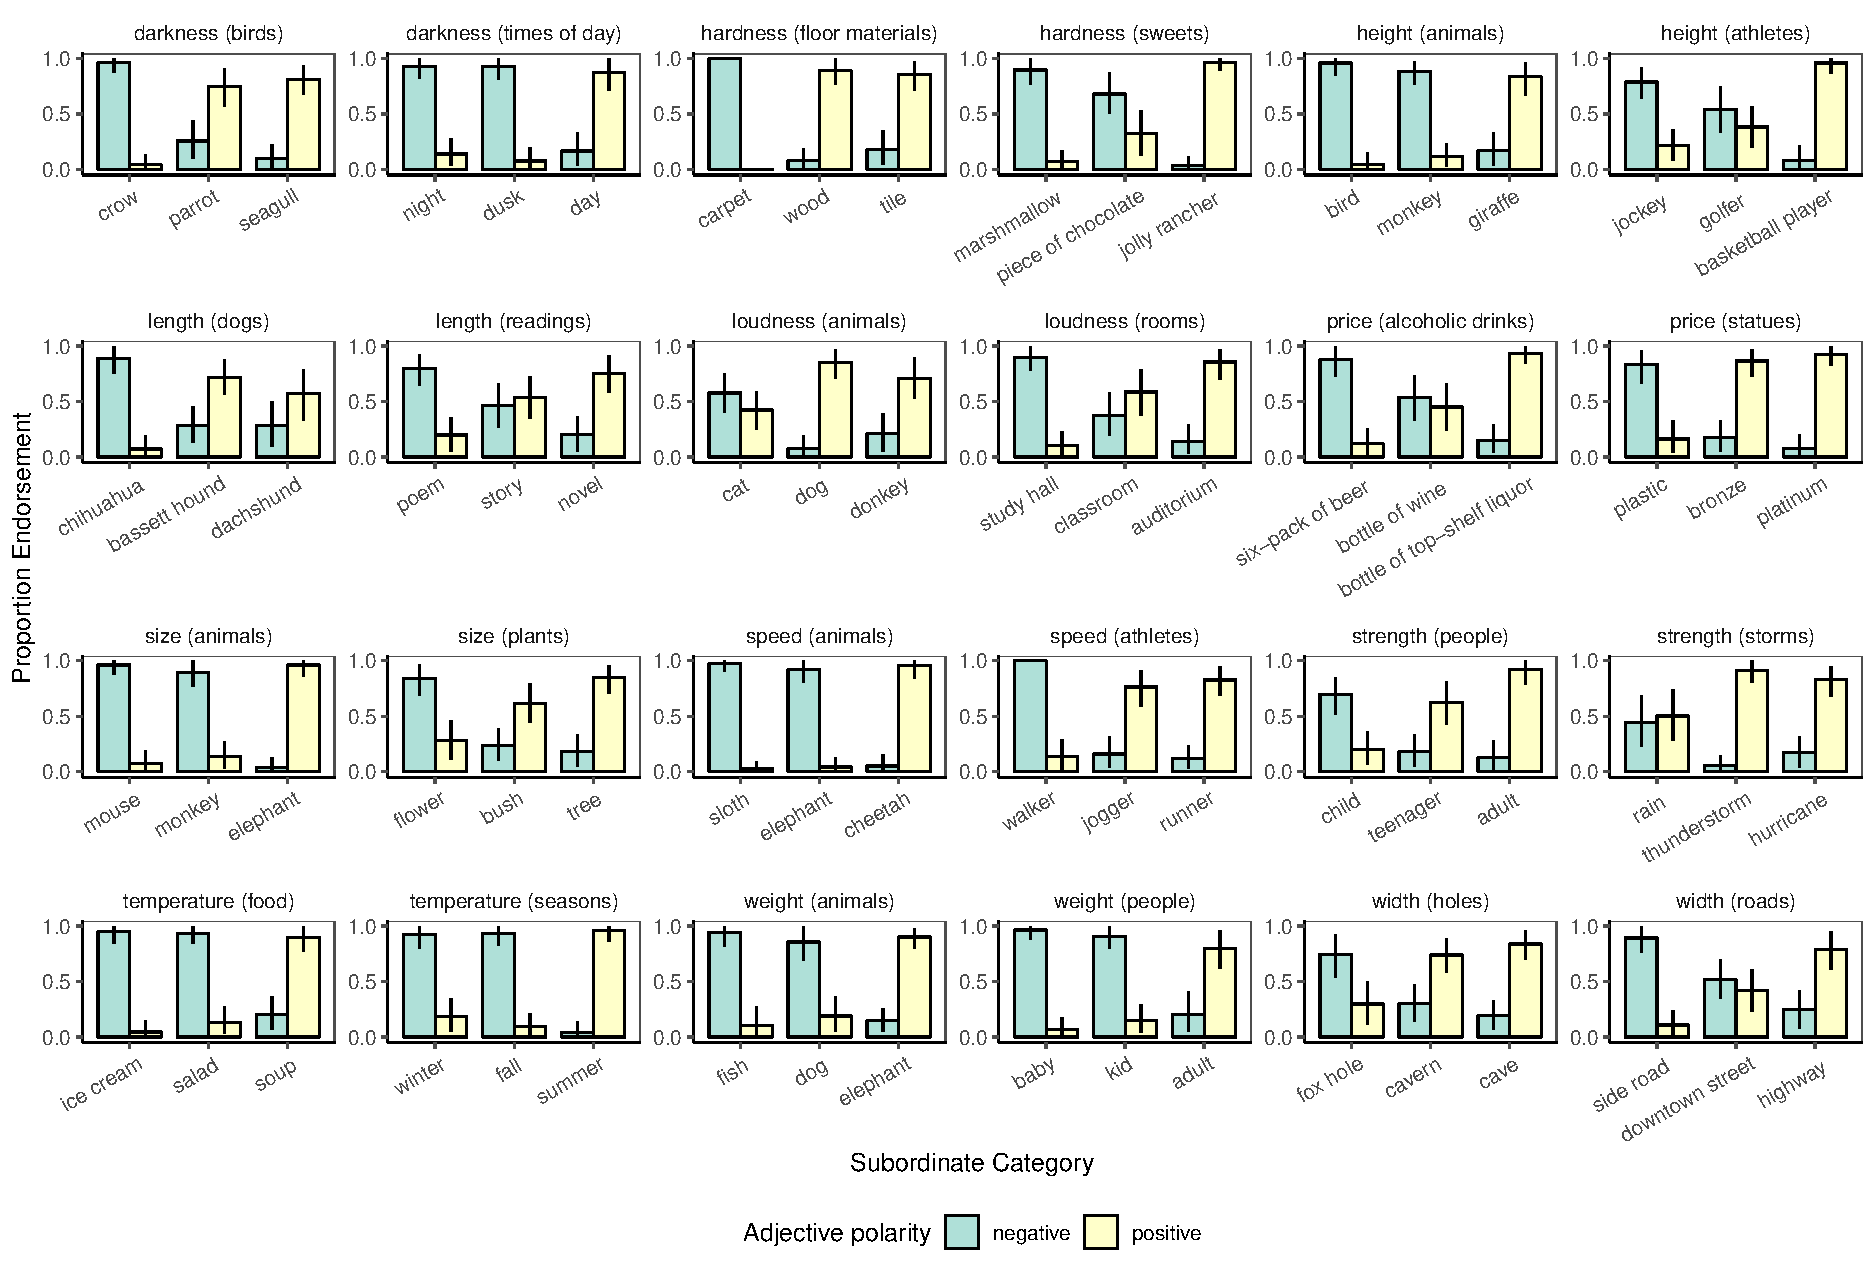
\includegraphics[width=\textwidth]{figs/bars_adj_finalExpt_pilot_byItem.pdf}
%{\centering 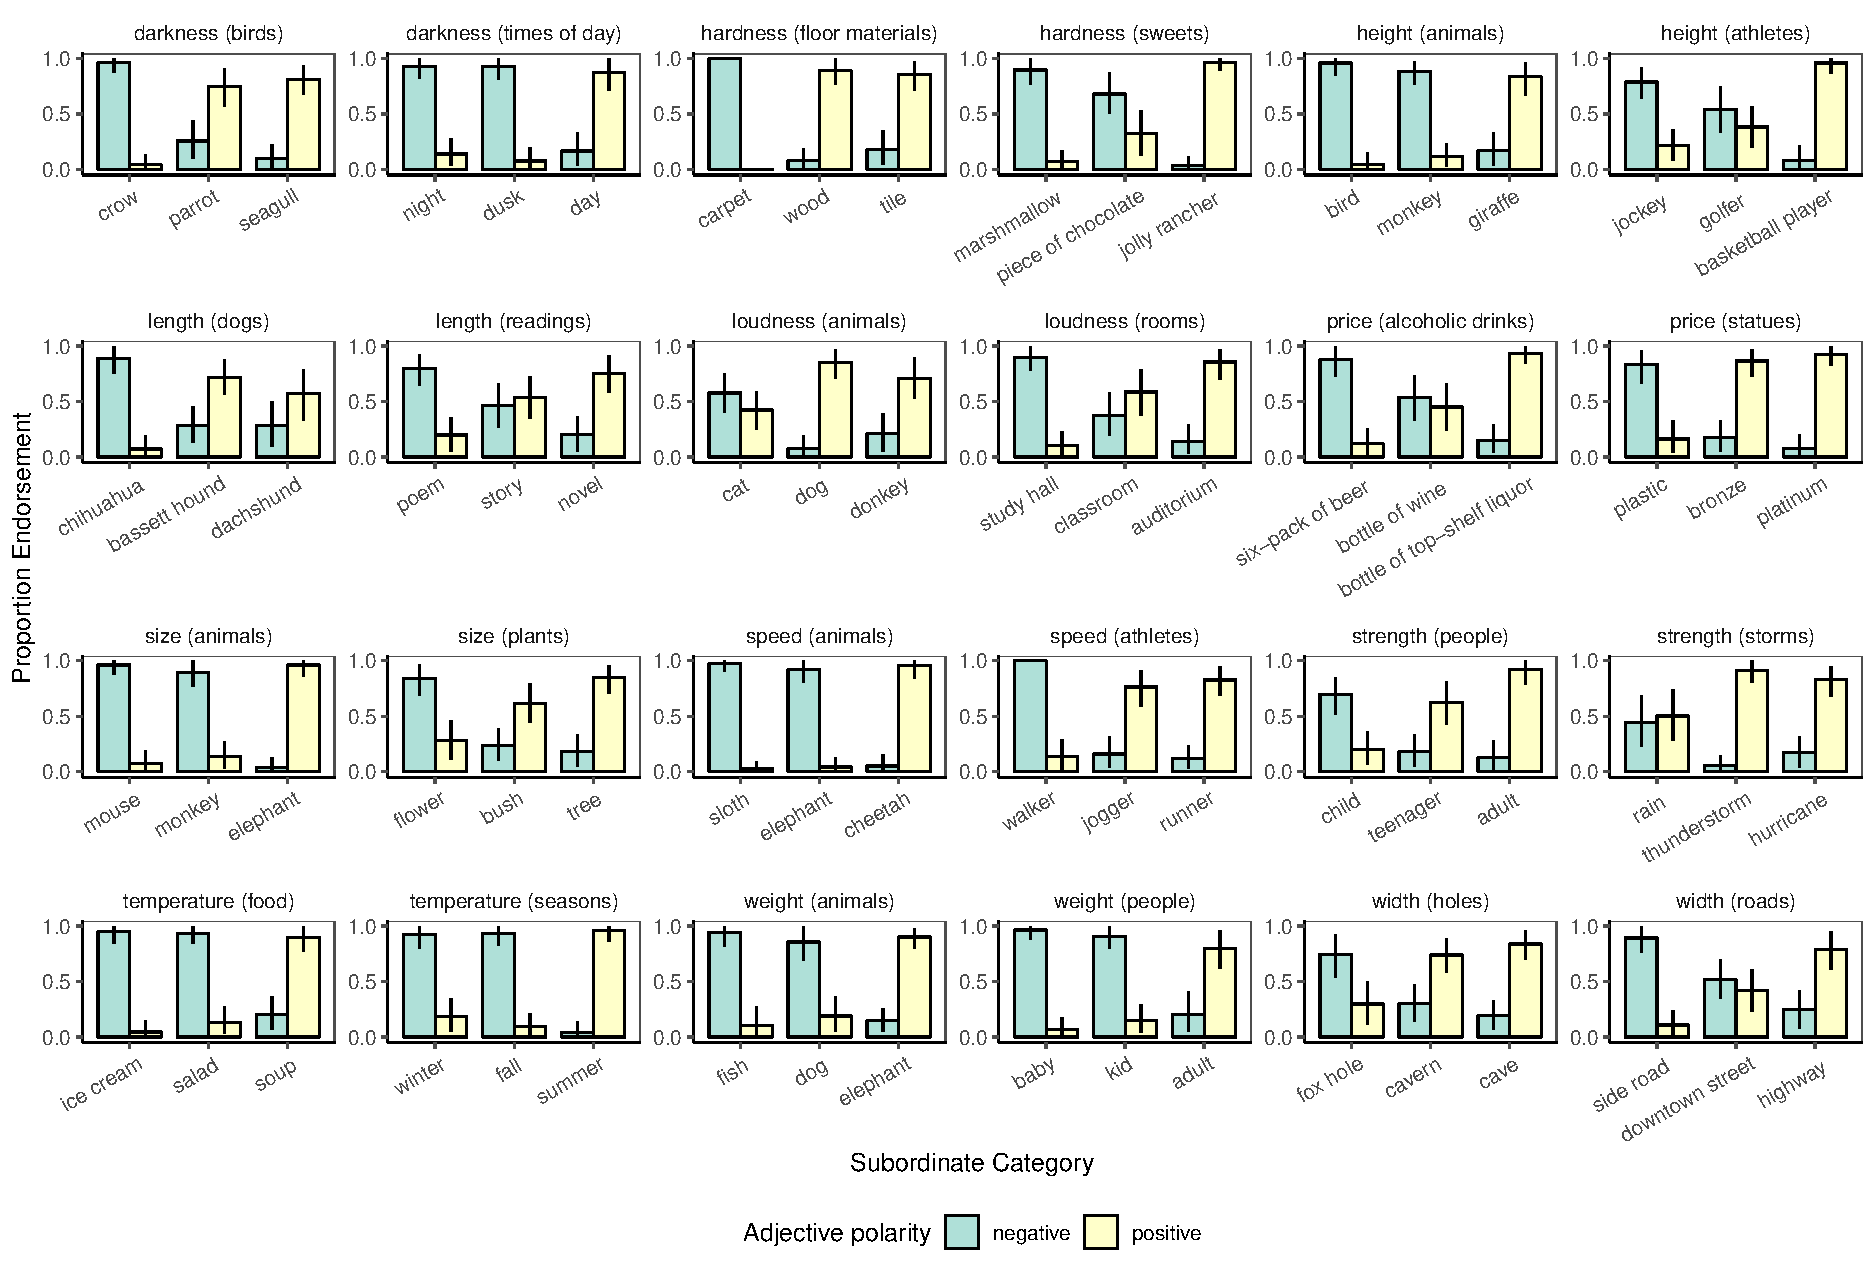
\includegraphics{figs/bars_adj_finalExpt_pilot_byItem} }
\caption{Experiment 3 (Adjective Endorsement) results for a subset of the items.}\label{fig:adjEndorseItems}
\end{figure}

\subsection{Bayesian data analysis model supplementary details}

Previous modeling papers in the RSA tradition empirically elicit world knowledge $P(x)$ through prior elicitation tasks.
Such tasks typically involve estimating numerical quantities or making probability judgments, for which the participant must have relevant knowledge concerning the units of measure (e.g., prices in dollars) and/or for which complicated linking functions are designed to relate latent probabilities to the estimation data \cite{Franke2016}. 
In order to estimate world knowledge $P(x)$ for our large, heterogeneous set of items, we take a different approach.

\subsubsection{World knowledge priors}

In our model, world knowledge is represented by probability distributions over degrees (e.g., heights).
Comparing interpretations of the same adjective across different comparison classes is an inherently relative judgment; thus, only the relative values for the degrees affect model predictions. 
Therefore, we fix each general (basic/superordinate) class in each domain to be a standard normal distribution---$P(x \mid c = c_{general}) = \mathcal{N}(0, 1)$---and assume the specific (subordinate/basic) priors to also be Gaussian distributions---\(P(x \mid c = c_{sub}) = \mathcal{N}(\mu_{sub}, \sigma_{sub})\); the subordinate priors thus have standardized units.
These parameters vary by the category $k = c_{sub}$ as well as the degree scale (e.g., height vs. weight).
We infer the plausible values of the parameters governing the subordinate priors from the data.

%This model with uncertainty around the parameters of the world knowledge priors is overparameretized, however, with respect to the comparison class inference data. The data from the comparison class experiment (Task 2) is insufficient to reliably estimate the model parameters governing the world knowledge priors. 
To constrain the world knowledge parameters, we use the same RSA architecture to predict additional data about a related Adjective Endorsement task (Expt.~3). 
In the Adjective Endorsement task ($n=375$), participants are asked to judge whether a gradable adjective (e.g., \emph{warm} or \emph{cold}) would be true of a hypothetical member of a specific category relative to the basic- or superordinate level category (e.g., \emph{You step outside during the winter. Do you think it would be warm relative to other days of the year? ...cold relative to other days of the year?}). 
That is, we have participants judge the truth or falsity of adjectives when the comparison class is explicit (see Supplementary Information for full experimental details).

To model the adjective endorsement data, we modify our comparison class inference RSA model by removing comparison class uncertainty from the model (since the task provides the comparison class explicitly) and, following \citeA{Tessler2019psychrev}, model sentence endorsement as a speaker deciding whether or not to produce the adjectival utterance to the listener: $S_{1}(u \mid k) \propto \exp{(\alpha_2 \cdot {\mathbb E}_{x\sim P_{k}}} \ln{L_0(x \mid u)})$, where $L_0(x \mid u)$ is given by Eq. \ref{eq:L0}. 
The speaker's decision rule marginalizes over their beliefs about the property value of the referent in the category (e.g., the speaker doesn't know the exact height of the referent, but knows that the referent is a basketball player and averages over plausible heights of basketball players: $x\sim P_{k}$).


%\newpage
%\section{Appendix}
%
%
%%Gradable adjectives like \emph{warm} and \emph{cold} are vague
%%descriptions of an underlying quantitative scale (e.g., temperature).
%Classic semantic theories posit the meaning of gradable adjectives to simply be that the scalar degree $x$ (e.g., temperature) is greater than or less than a contextually-supplied standard of comparison  \(\theta_c\): \([\![u_{pos}]\!] = x > \theta_c\), for positive-form adjectival utterance \(u_{pos}\) (e.g., warm) and \([\![u_{neg}]\!] = x < \theta_c\), for negative-form adjectival utterance \(u_{neg}\) (e.g., cold).
% Lassiter \& Goodman (2013) model the context-sensitivity of these adjectival utterances using threshold semantics, where
%the threshold is probabilistically set with respect to a comparison class \(c\) via pragmatic reasoning :
%
%\begin{align}
%L_{1}(x, \theta \mid u, c) &\propto S_{1}(u \mid x, \theta) \cdot P(x \mid c) \cdot P(\theta) \label{eq:L1} \\
%S_{1}(u \mid x, \theta, c) &\propto \exp{(\alpha_1 \cdot (\ln {L_{0}(x \mid u, \theta, c)} - \text{cost}(u)))} \label{eq:S1}\\
%L_{0}(x \mid u, \theta, c) &\propto {\delta_{[\![u]\!](x, \theta)} \cdot P(x \mid c)} \label{eq:L0}
%\end{align}
%
%Eqs. \ref{eq:L1} - \ref{eq:L0} are the Rational Speech Act mode  Lassiter \& Goodman (2013). 
%In this model, a pragmatic listener \(L_1\)
%tries to resolve the degree \(x\) (e.g., the temperature)
%from the adjectival utterance she heard \(u\) (e.g., ``it's warm''), by assuming the utterance came from an approximately rational Bayesian
%speaker \(S_1\) trying to inform a naive listener \(L_0\), who in turn
%updates their prior beliefs \(P_c(x)\) via an utterance's literal meaning
%\([\![u]\!](x, \theta)\).
%Formally, the literal meaning is represented by the
%Kronecker delta function \(\delta_{\mbox{ $[\![ u ]\!]$}(x, \theta)}\)
%that returns probabilities proportional to \(1\) when the utterance is
%true (i.e., when \(x > \theta\)) and \(0\) otherwise.
%The key innovation used for modeling gradable adjectives is to have uncertainty over the
%semantic variable---the threshold \(\theta\) (Eq. \ref{eq:L1}). In
%Lassiter and Goodman (2013)'s model, \(\theta\) comes from an improper uniform
%prior distribution over thresholds defined over the real numbers and is resolved by the
%listener reasoning about the different thresholds a speaker might be
%using \(S_{1}(u \mid x, \theta)\) as well as the probabilities of
%different states of the world \(P(x \mid c)\) (e.g., different
%temperatures). Assuming the adjective adds some cost to the speaker's
%utterance (Eq. \ref{eq:S1}), the meaning of a gradable adjectives (e.g.,
%``warm'') is resolved by the pragmatic listener to mean something
%like ``significantly greater temperature than one might expect''
%(Lassiter \& Goodman, 2015). Critically, what ``one might
%expect''---the prior distribution over temperatures \(P(x \mid c)\)---is
%always with respect to some comparison class \(c\) (Eqs. \ref{eq:L1} \&
%\ref{eq:L0})
%

\end{document}
